\newpage
\section{Experiments and Evaluation}
\label{sec:experiments}

The main goal of our thesis was to compare different state of the art algorithms and to combine machine learning techniques to gain a deeper understanding of what is necessary and what is possible in order to achieve the best results based on an initial data set and certain evaluation targets that one wants to find. In this chapter we explore our procedure from the initial dataset that we work with to the final comparison of the results that we produced.

\subsection{Introduction / Procedure}

At first we did an initial data analysis and created a naive approach that allowed us to gain further insight into our data as a whole and to create a proof-of-concept whether the assumptions we had about our data are justifiable. 
We then continued to use actual machine learning algorithms implemented into the WEKA toolkit. As part of this we discuss our execution plan, the different features we combined, executed and evaluated and the way we gathered and compared the results.

In order to have data that the algorithms can use directly and to avoid outliers or false cases we combined statistical analysis together with data preparation to convert our raw dataset into a reasonably filtered and correctly formatted set. As discussed in Section~\ref{subsec:proposed_solution} we used a decision tree algorithm, a Naive Bayes algorithm and a multilayer perceptron to train and evaluate our dataset. After improving the process and gathering the results we compared the different execution plans and algorithms and analyzed the impact of different design decisions of our approach.

We have used Groovy to implement all the data analysis, preprocessing and evaluation tasks that we have implemented ourselves. Due to the JVM-based nature of Groovy we could easily and directly interact with WEKA, but we also had all the advantages of rapid prototyping, dynamic types, easy scripting and all the other advantages that Groovy provides on top of Java. 

\subsection{Data Set / Data Analysis}
\label{subsec:data_set}
The first step to getting started with machine learning is to know about the data and the underlying domain associated with it. Machine learning is not an oracle where data can be inserted and the computer spits out everything you ever wondered about. Careful analysis and domain knowledge are crucial. 

\subsubsection{Data Set}
Our data was gathered over months from active user of an Android smartphone app. The app (Farplano) gives the user an overview of the current timetable of train and bus stations close to him. The timetable is based on an open data set from SBB (Swiss Railway company). The app contains features such as automatic geolocation, full route information of bus and train lines, arbitrary connection planning and many more. In addition to that it also allowed the user (with an opt-in feature) to track his position and anonymously store the stations with timestamps that he passes. We worked on this gathered dataset from hundreds of users over many months. The raw data contains an entry for every station the user passes. A single data entry contains the following data points:
\begin{itemize}
	\item Anonymized User ID (a 9-character String)
	\item Station ID (a 7-character String)
	\item Timestamp
\end{itemize}
The information contained in the raw dataset is relatively trivial. In order to be able to successfully predict the future location of a user we combined multiple entries to get further information. As a first step we split up the data set into separate subsets for each user. We also sorted the entries by timestamp to have a chronological view of all the events as they actually happened.

Remark: We have purposefully left out global state and information about usage patterns, mostly due to the added complexity as well as performance reasons. However this might be something that could be analyzed and included in future work. 

\subsubsection{Data Analysis}
To get a basic understanding of what kind of data we have and to be able to reason about our data set we created a number of charts, based on the features we will later use for the machine learning algorithms. 

As a first analysis we looked at how the data is distributed by time and day, as can be seen in the following two charts.

\begin{figure}[!ht]
	\caption{Distribution by Time of Day}
	\centering
	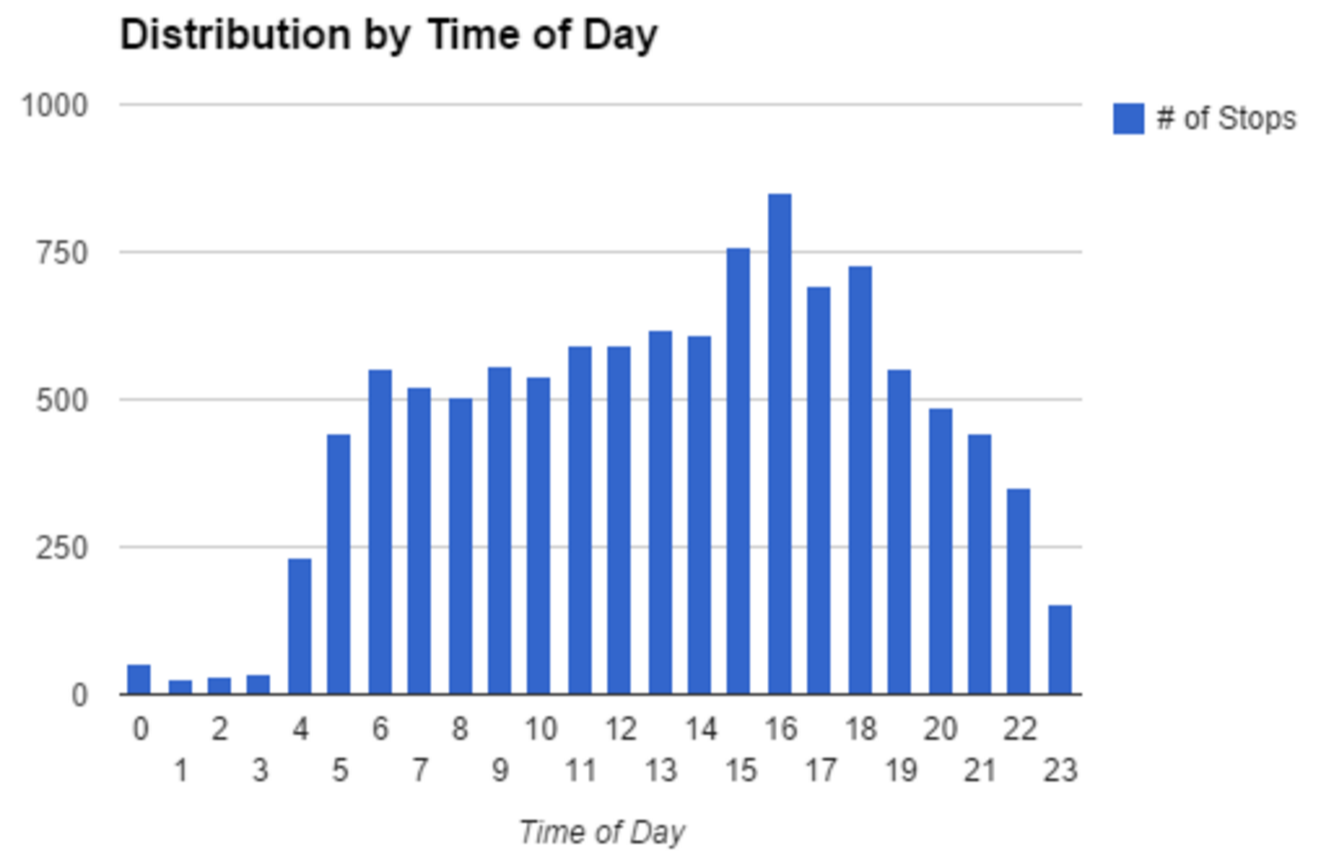
\includegraphics[width=1.0\textwidth]{charts/distribution_time_of_day}
\end{figure}

\begin{figure}[!ht]
	\caption{Distribution by Day of Month}
	\centering
	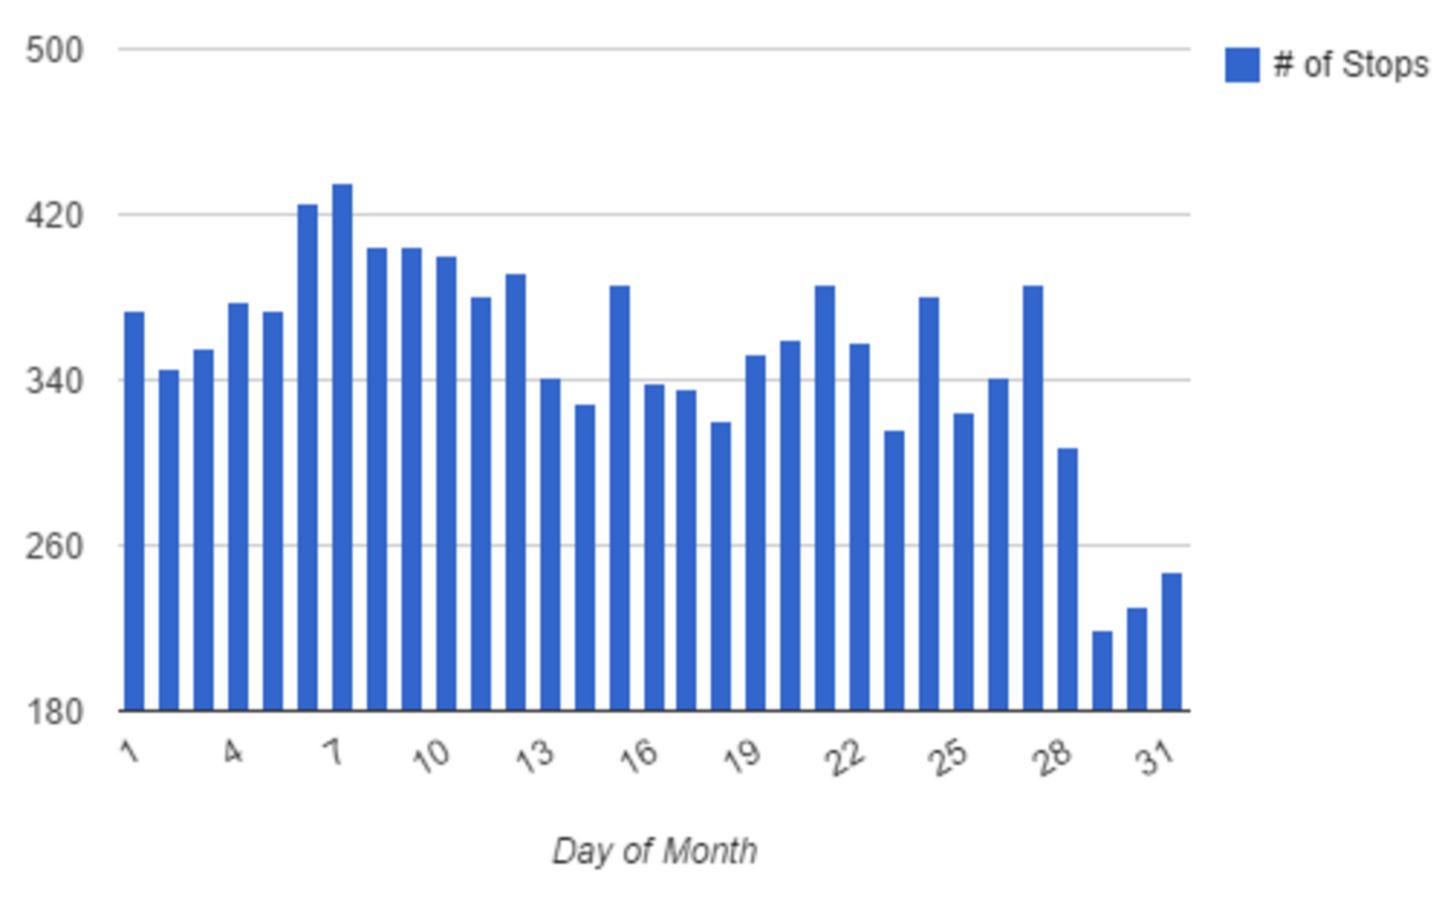
\includegraphics[width=1.0\textwidth]{charts/day_of_month_distribution}
\end{figure}

As we expected we encountered the highest usage during commuting hours, especially in the afternoon. The distribution gets significantly lower as midnight is approached. During the night we have very few gathered data points. The only somewhat surprising point was that the commute hours in the morning didn't produce as high a peak as the hours in the afternoon. However the fact that the data from the app is gathered voluntarily and the app needs to be open to collect data might explain these small inconsistencies.

The distribution by day of month didn't really produce significant insight. The fact that in the end of the month the number of stops are significantly lower is due to fewer months having 31 days. The data set isn't normalized against this and will therefore include such issues. However what this tells us is that the day of month might not be a good indicator. It would be worth exploring the difference between weekday and weekend-day. Since commuting behavior is generally vastly different on weekends as on weekdays this comparison might lead to deeper and more succinct insights.

\begin{figure}[!ht]
	\caption{Number of Stations per User}
	\centering
	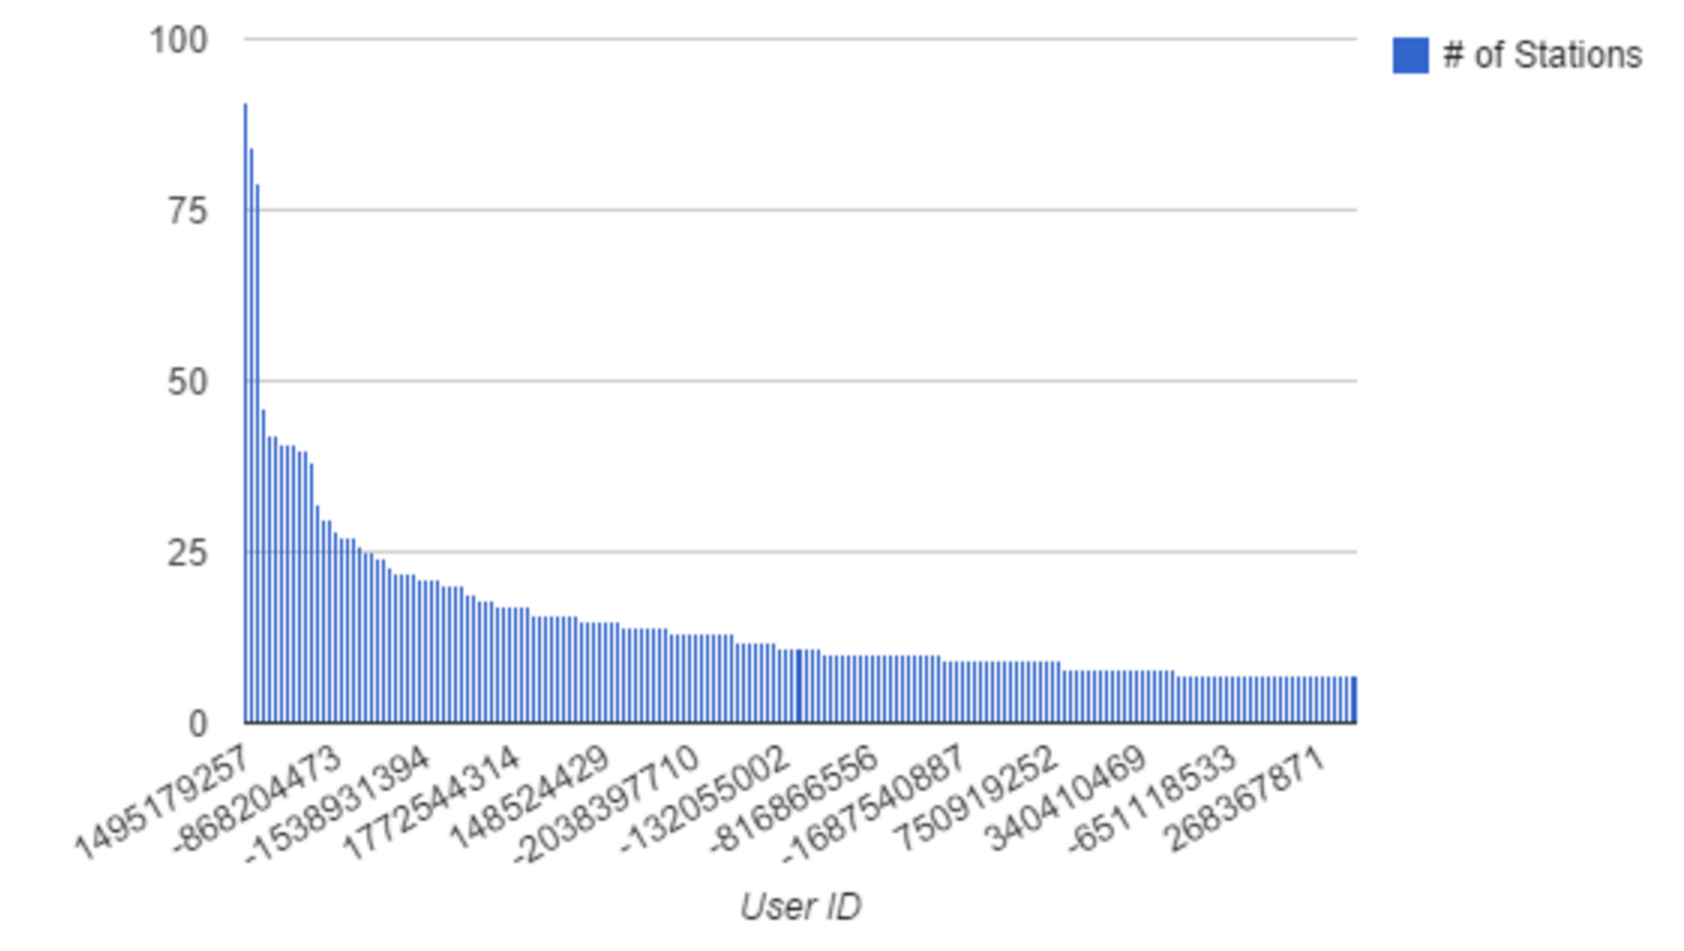
\includegraphics[width=1.0\textwidth]{charts/different_stations_per_user}
\end{figure}


\begin{figure}[!ht]
	\caption{Number of Stops per User}
	\centering
	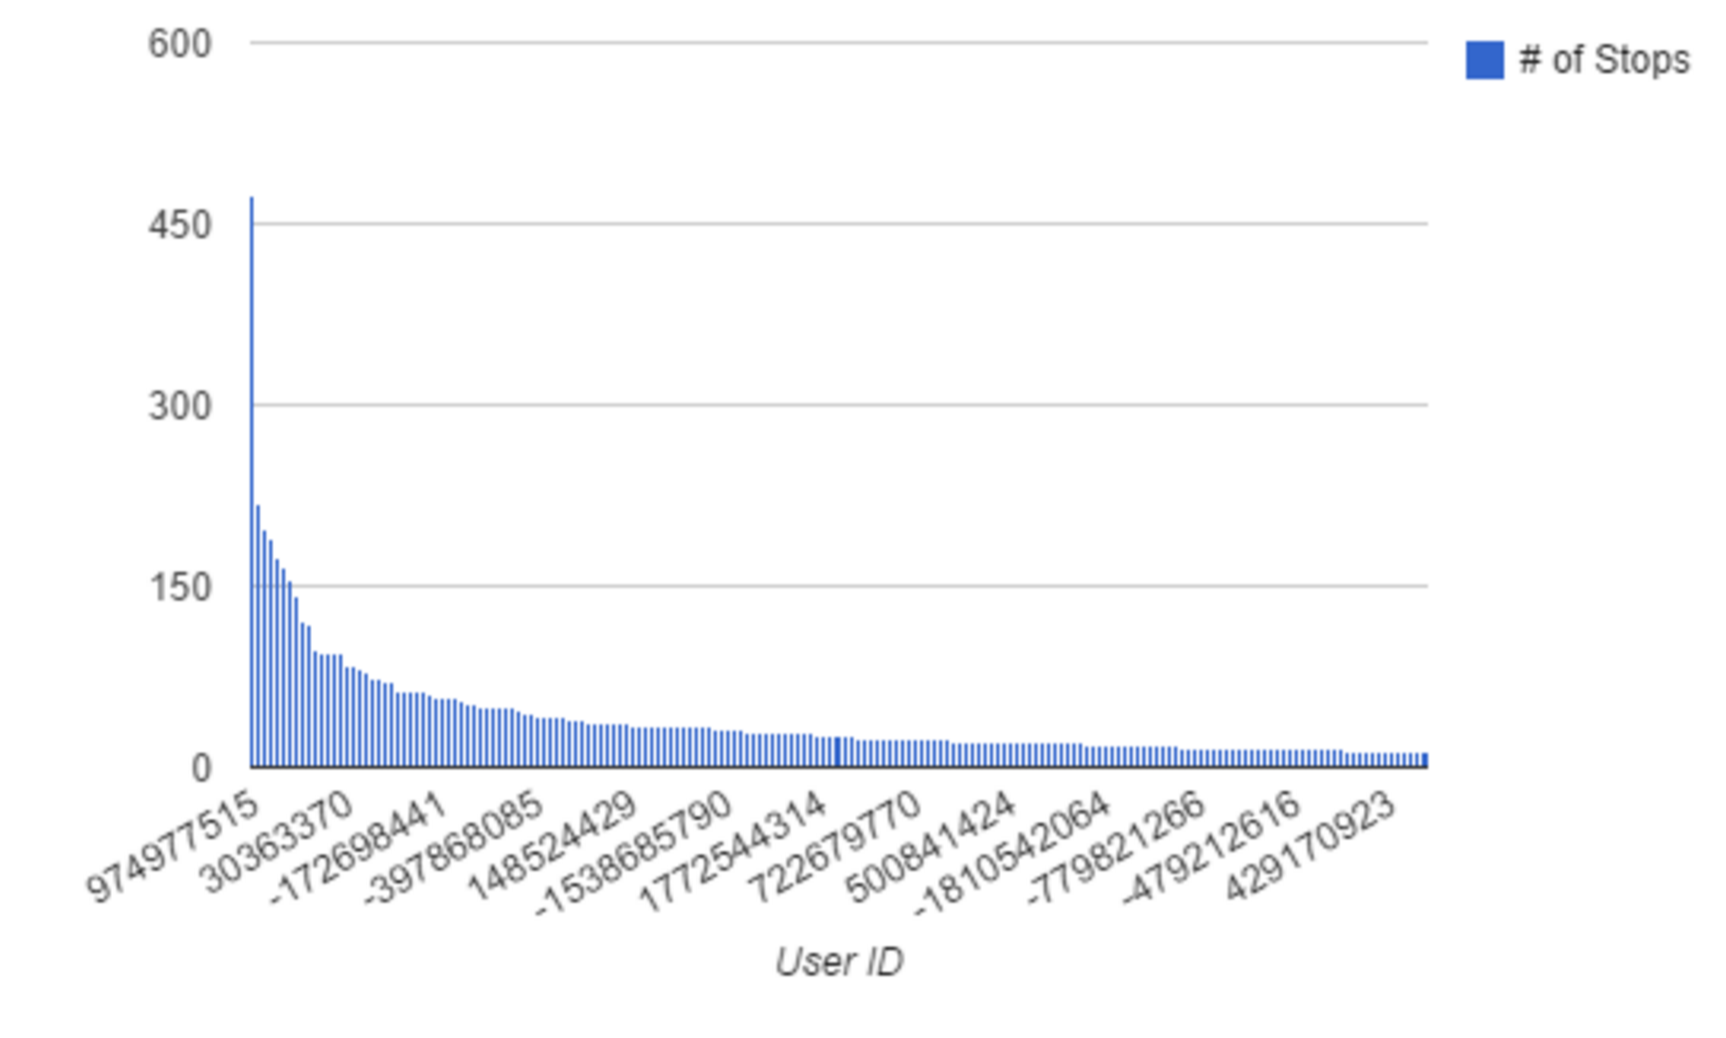
\includegraphics[width=1.0\textwidth]{charts/stops_per_user}
\end{figure}

\begin{figure}[!ht]
	\caption{Number of Users per Station}
	\centering
	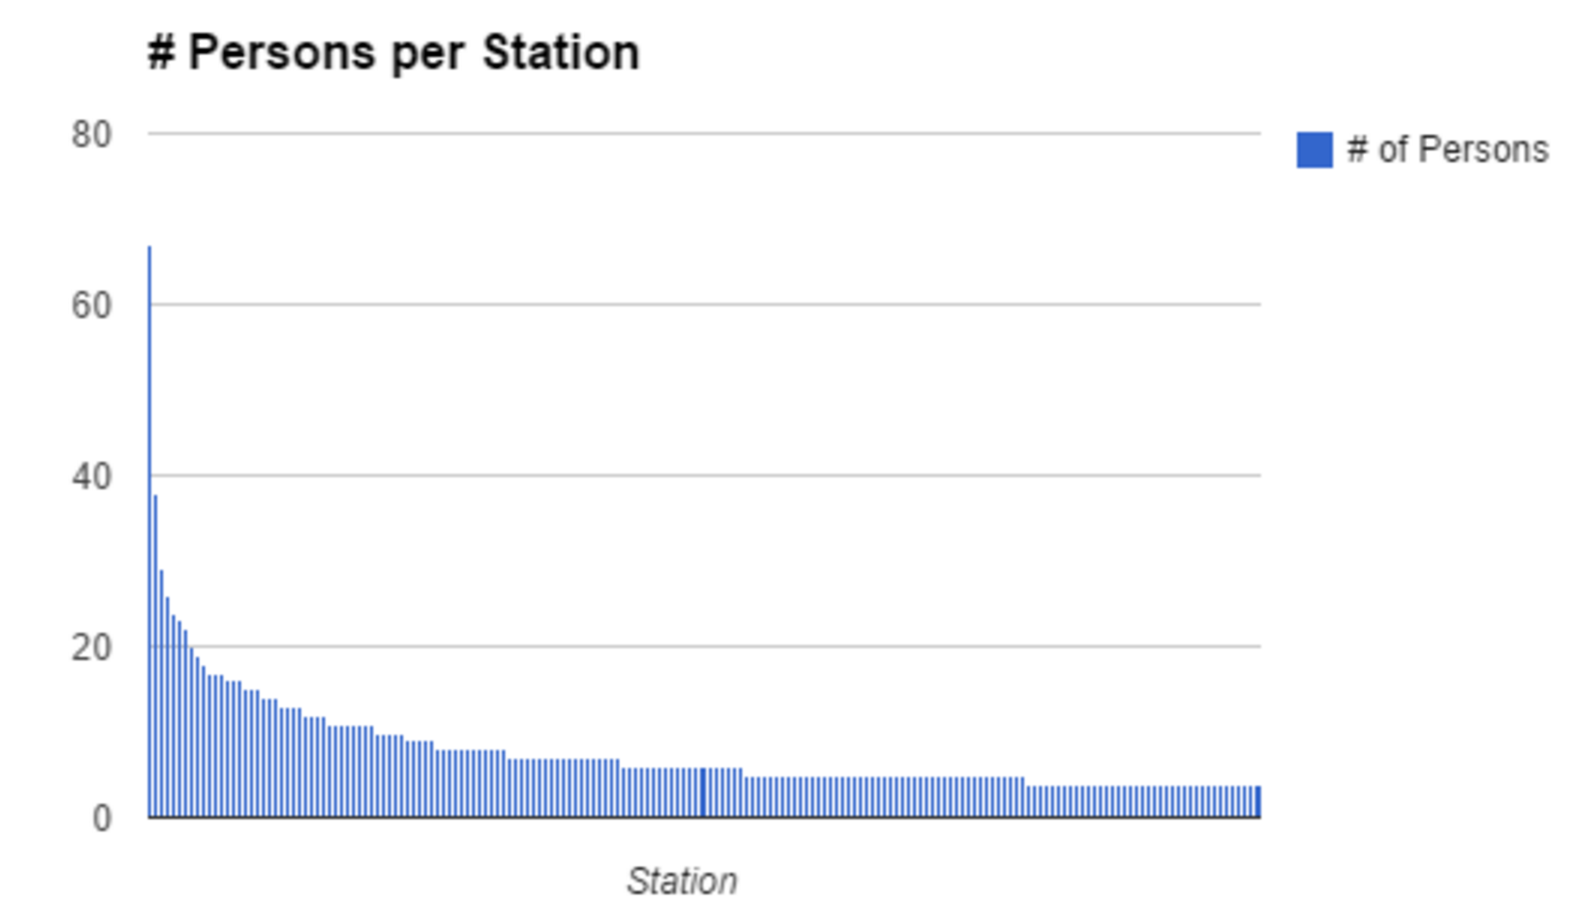
\includegraphics[width=1.0\textwidth]{charts/persons_per_station}
\end{figure}

A vastly more interesting and also challenging conclusion can be drawn from comparing the users with the stations they frequent and how often they stop at stations. As we expected there are a few users that have amassed a lot of data and then there is a long tail of less frequent users. The same statistic also applies to the number of stations and the number of stops that have been gathered for a user. What we already realized here is that it will be very difficult if not impossible to get a good prediction for the users tailing the statistics, simply because there is just not enough data available. In some edge cases where a user really only has 2 or 3 stops that he regularly frequents this might work, otherwise it will just be stabbing in the dark to get a reasonably good prediction. One or two outliers from such a user could possibly mix up the complete prediction process. It seems sensible to cut the dataset into high- and low-frequency users and discard the latter. The exact boundary or whether it will be flexible to a certain degree will have to be tested by trial and error, however if we would not cut the low-frequency user out of our comparison tests it might greatly change our conclusions and the effectiveness of our process.

\begin{figure}[!ht]
	\caption{Distribution of Stops per Station}
	\centering
	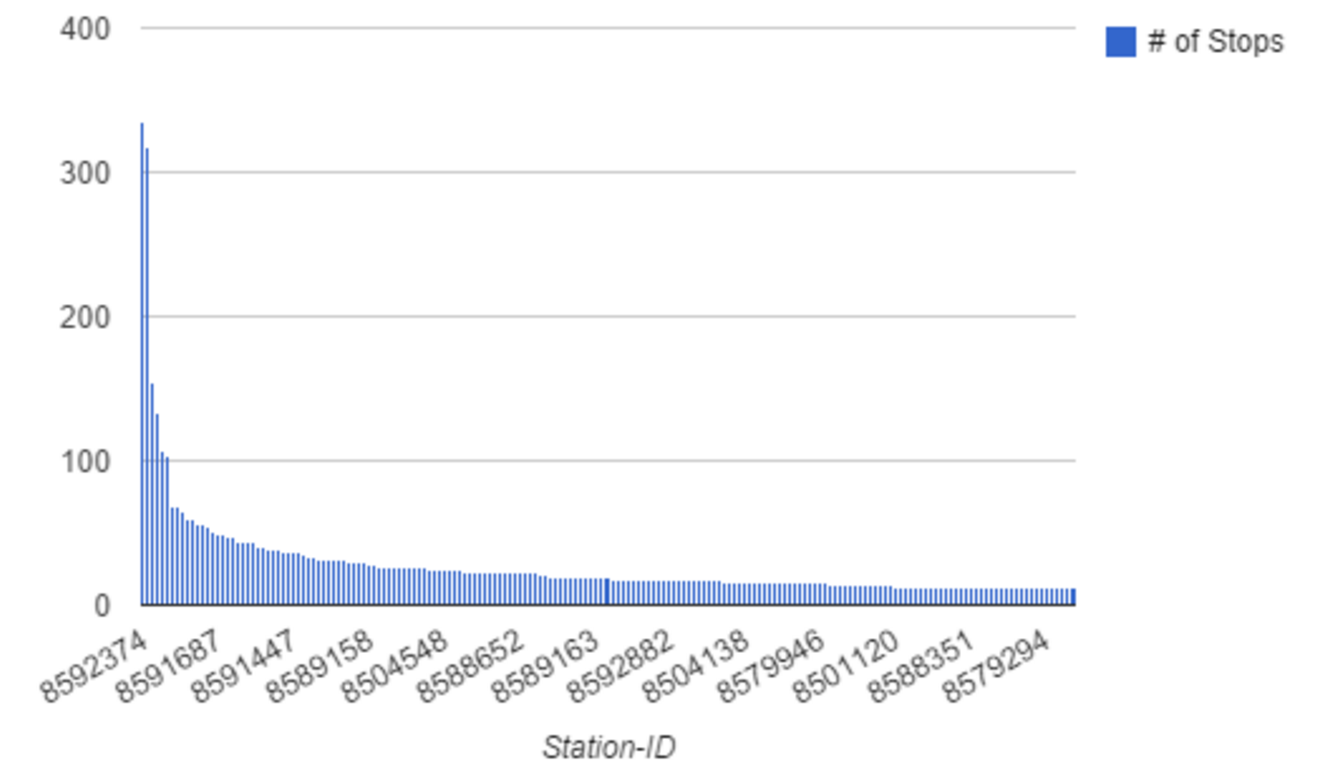
\includegraphics[width=1.0\textwidth]{charts/distribution_stops_by_station}
\end{figure}

\begin{figure}[!ht]
	\caption{Average number of accesses per station by users}
	\centering
	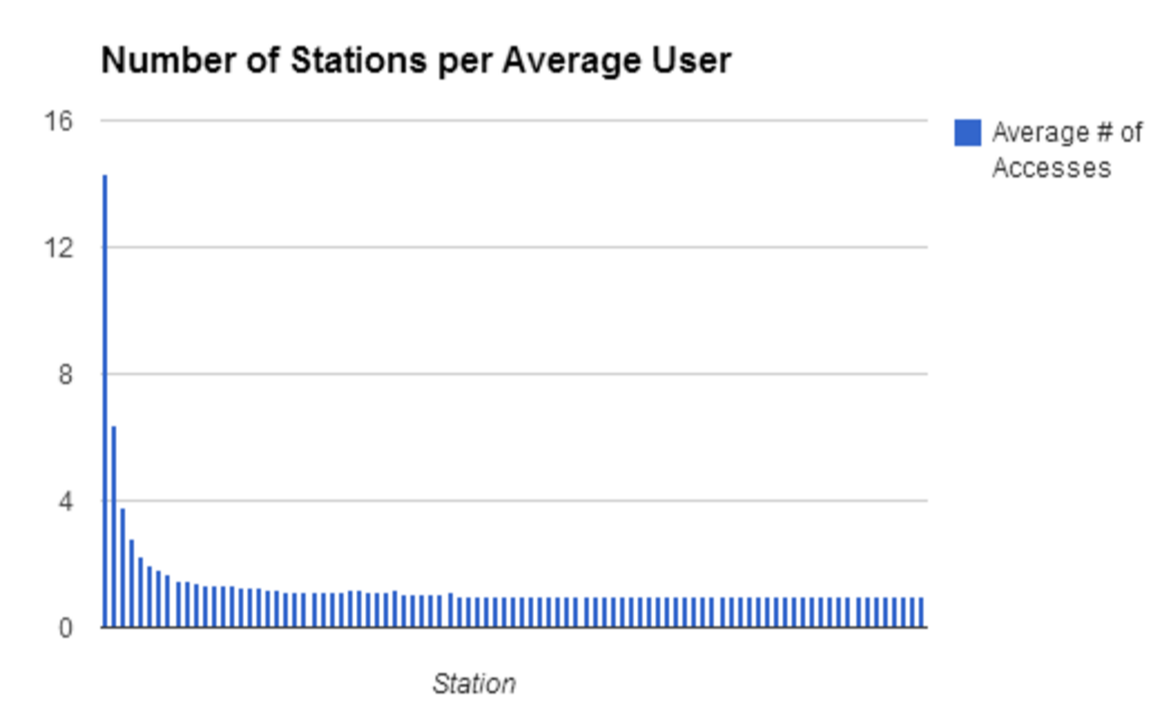
\includegraphics[width=1.0\textwidth]{charts/number_stations_average_user}
\end{figure}

A similar conclusion can also be drawn by the more averaging figures that we created. It also shows a relatively small set with a lot of data and a long, small tail. Combined with the previous conclusions this strengthened our approach of doing statistical analysis and preparing the data set to remove data points that will skew our result. The types of preparation, analysis and restrictions we've imposed on our data set are described in detail in ~\ref{subsubsec:data_preparation}

\subsection{Naive Approach}

As a first approach we wanted to create a reasonable starting point to work with our data set. For this we created a naive approach in how we first measured and analyzed our data. 

We took our complete data set without doing any statistical analysis or restriction and created a graph for each user. The graph consists of nodes and edges. Each node represent a station and we drew an edge from a node to another node if the destination was the immediate successor of a station in our data set. This resulted in a graph that looked as described in Subsection \ref{subsubsec:web_gui} and that reflects how the users travel across the network of stations. Our guess was that since a user might generally take similar paths on his travels this would be reflected in the graph and could give us a good first estimate.

For the analysis we then looked at the node that was to be analyzed (assuming this is the node the user would currently be at) and just took the path with the most outgoing edges as our prediction. We then validated this against the ground truth that we had established previously, where we just ordered all the stops at the stations in chronological order. The expected prediction would therefore always be the station that appears next in chronological order for a user. 

This naive approach with all its known limitations and issues gave us a correct prediction of 45.7\%. We have purposefully chosen not to limit our data set or to put it under certain limitations. This obviously leads to a worse overall prediction and also to some wrong predictions that will be classified as correct, since our ground truth does not necessarily fully reflect the actual reality. However our goal was to start out with a reasonable estimate on the basis of our data set. We didn`t want to prematurely optimize issues away that wouldn`t really disturb our prediction models. With that approach we could start out from the very base of our prediction and then analyze the effects that statistical optimizations and a better preparation of our data set have. Thanks to the naive approach that we created we could make sure that what we analyzed with machine learning techniques and the statistical analysis and preparations that we did were actual optimizations and gains in precision.

\subsubsection{Web GUI, Visual Representation}
\label{subsubsec:web_gui}
Since we were aiming for a reasonable starting point and a general look into our data set we thought it makes sense to also create a visual representation, at least for that first step, before going further into detail. It should allow us to look at individual users and analyze the naive graph that was created for said user. Having such a visual representation helps us in reviewing data for user, seeing at how the data is distributed and can also aid in the analysis of any issues with the data. The resulting graph that was provided by our Web GUI can be seen in Figure \ref{figure:web_gui_graph}. We can see all the nodes the user has visited and the relations as well as the amount of relations between each of these nodes. The Web GUI also allowed us to move the nodes around in order to de-clutter the graph, as well as to enable or disable certain nodes. This is especially useful when a user has a huge number of nodes and we only want to look at a certain part of the users graph.

\begin{figure}[!ht]
	\centering
	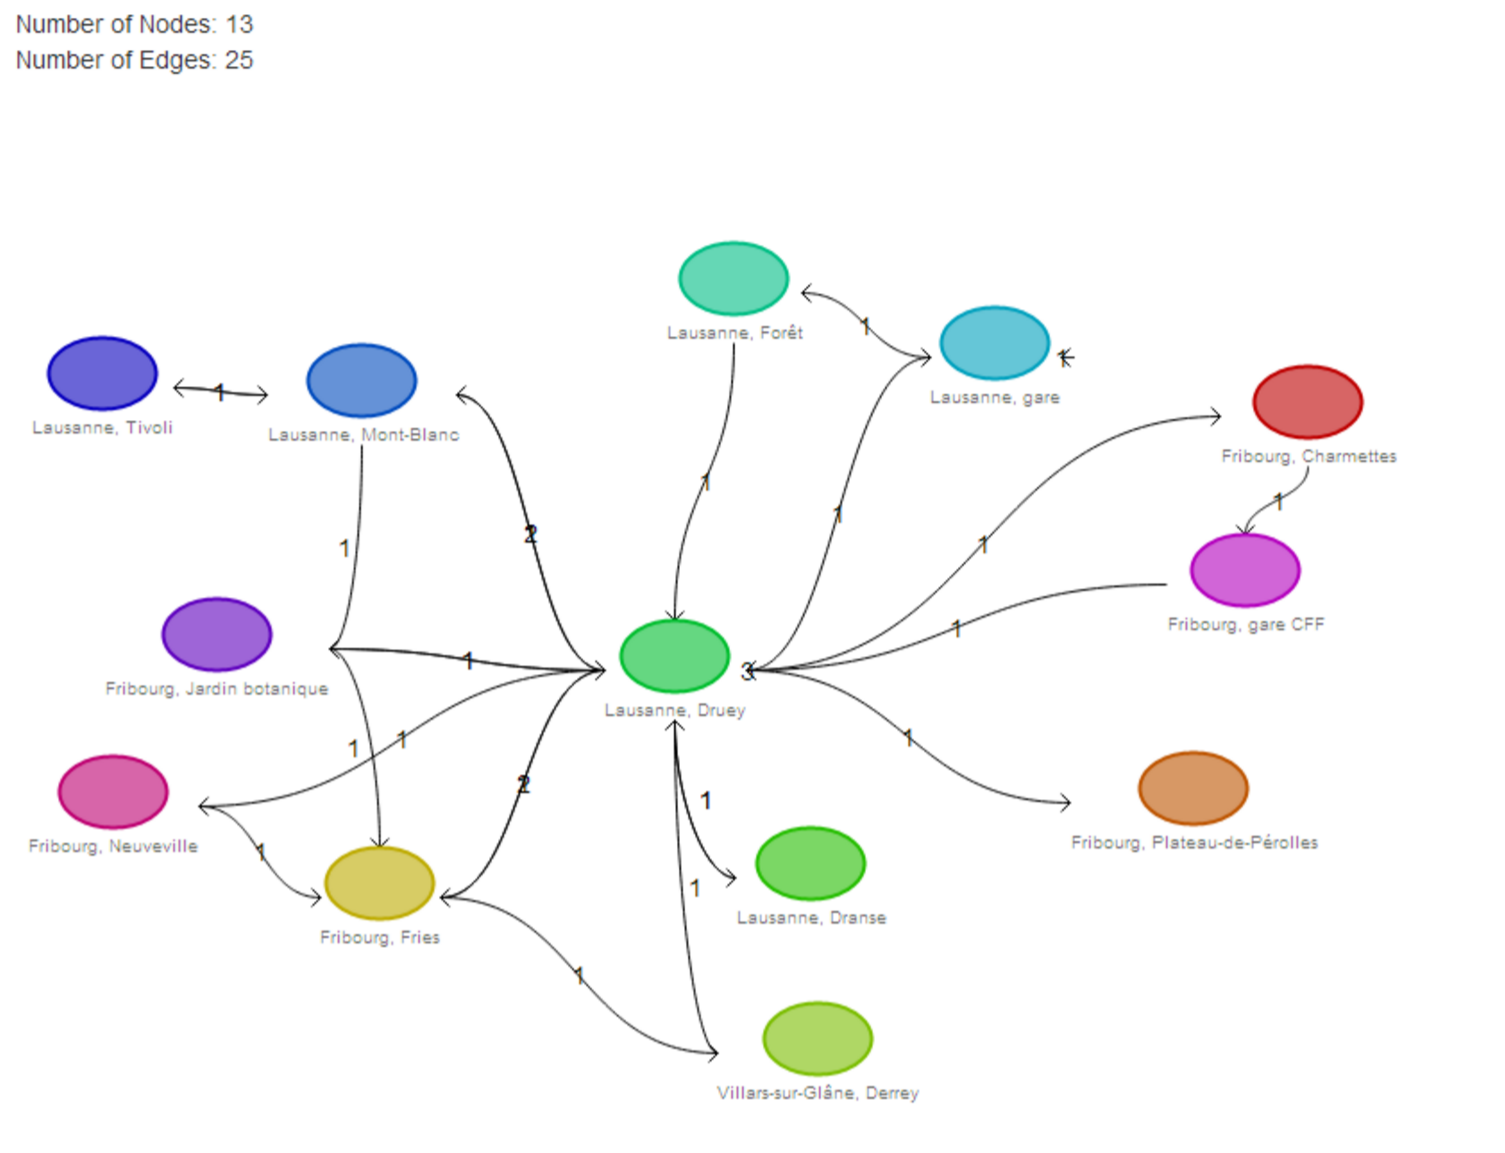
\includegraphics[width=1.0\textwidth]{images/web-gui}
	\caption{Generated Graph in Web GUI}
	\label{figure:web_gui_graph}
\end{figure}

\subsection{Machine Learning Preparation}
\label{subsec:machine_learning_results}
As outlined before applying machine learning techniques to our problem was the main goal of our thesis. After having gathered insights into our dataset by statistical means and by looking at the dataset with a naive approach we started working on machine learning. We laid out our execution plan, defining what and how we want to test the different algorithms on our dataset, what kind of algorithms we'd use and how we evaluate and compare the results. The following sections are the result of carrying out these plans.

\subsubsection{Execution Plan}
The reason to have a proper execution plan is to have a reproducible way of evaluating the features with different classifiers and reason about the gathered results. 

The classifiers that we use are already described in a theoretical manner in section \ref{subsec:proposed_solution}. We have used a decision tree classifier and a naive Bayes classifier both provided from WEKA. As a classifier with back propagation we have used a multilayer perceptron also provided by WEKA.

To test the accuracy of each of the classifiers trained with different features we are using the F1 score. The F1 score considers both the precision and the recall. In information retrieval the precision is defined as "How many selected items are relevant?" whereas the recall is defined as "How many relevant items are selected?". The combination of both precision and recall gives quite a good approximation of the accuracy of a classifier and allows us to easily compare the different results with each other. Mathematically the F1 score is defined as 
\begin{equation}\label{equation:F1Score}
F_{1} = 2 \cdot \frac{precision \cdot recall}{precision + recall}
\end{equation}

The F1 score is also called traditional F-measure or balanced F-score, as it's the harmonic mean of precision and recall and thus weighs both measurements equally.

We are using the precision, recall and F1 score directly to compare the different executions and to analyze their results. However we also split up the result set to compare the precision/recall/F1 for the number of most frequent stations used as well as for different types of users (frequent/non-frequent). With that analysis we should be able to see how the prediction for different usage patterns and types of users are influenced by our classifiers.

The features that we have been able to identify from our data set and that we have worked with are the following:
\begin{itemize}
	\item Current Station
	\item Day of Week
	\item Hour of Day
	\item Minute of Hour
	\item Weekday or Weekendday
	\item Previous Station
	\item \textbf{Next station} (to be predicted)
\end{itemize}

The current station can directly be deduced from the gathered data. The same can be done thanks to the timestamp for the day of week, hour of day, minute of hour and the weekday/weekend flag. For the previous station we had to do some calculation as well as some assumptions about the data. The way we have prepared the previous station is described in more detail in section \ref{subsubsec:data_preparation}.  

The next station is the feature that we will be predicting with our algorithms. It is also called our ground truth. We know that our ground truth does not necessarily correspond to the actual reality, but it is the closest assumption we can make with the data and the resources we have at hand. Improving the ground truth would require either the actual implementation of the prediction into the Android app and letting the user give feedback on the prediction or sifting through the data manually and analyzing whether our ground truth makes sense given the user's behavior. Unfortunately both options are out of scope for this thesis, leading us to rely on our somewhat unreliable ground truth. The issue that could arise from that is that we optimize for a scenario that does not properly reflect reality and that would leave our results useless or require a lot of improvements for an actual real world use case.

In our execution plans we have used different combinations of the feature set above to train and then test the data set. We have always tried to predict the next station feature.


\subsubsection{Data Preparation / Statistical Analysis}
\label{subsubsec:data_preparation}
As part of the process to convert the raw data we have gathered into a WEKA-compatible format we also implemented the findings we gathered from our data analysis, from the naive approach and from the subsequent execution of our plans and the gathering of the results. We constantly improved the results of our predictions by taking the data with the preparation we had done so far, using the machine learning algorithms on the data and then analyzing the results. This process has not been a straightforward path where we knew what and how we needed to implement restrictions and enhancements on our data, but much more a continuous path, leading to small or significant improvements or decreases in precision. Based on the analysis of each step we took we were able to get a good precision, albeit at the cost described in this section. We outline all the transformations, restrictions and enhancements that we made on our data set here.

\paragraphtitle{Data Parsing} 
The first step in the process was to parse our data set. The data is available as a single large .csv files, each entry consisting of a line such as this:
\begin{lstlisting}
2015-11-26T23:25:46	path=/v1/training?stop_id=8592010	hashacc=595604002
\end{lstlisting}
Each line starts with the timestamp of the entry, followed by the api path that was made, the id of the station as well as a hash of the user. The relevant data for us is obviously the timestamp, the user hash (which is subsequently directly used as user id) and the station id. The api path is the same for every entry and is irrelevant for our use case. Directly during the import of the data into our model we separated each entry by user and discarded the entries that had an empty user id attached. There is always a timestamp and a station id available. We have also during the import already added the time-based additional fields to our model. These fields include the hour of day, minute of hour, the day of week and whether it's a weekday or weekend day. We also directly set the station id. The previous and next station are added in a later step. A model entry is internally represented by the following fields:
\begin{lstlisting}
public class ModelEntry {
	private String userId
	
	private Date timestampStart
	
	private int hourOfDay
	private int minuteOfHour
	private int dayOfWeek
	private Boolean weekday
	
	private String stationId
	private String previousStationId
	
	// This is the main thing to predict
	private String nextStationId
}
\end{lstlisting}
Now that we have completed the import of the raw data into our model we have a representation of every user with every entry that was gathered from said user. 

\paragraphtitle{Remove Duplicates}
The next step is to remove duplicate entries that are present in a user's entry list. Because the Android app responsible for gathering the data and sending it to the server periodically pulls the current location. If a user has to wait at a station for a few minutes it's possible that the app created not only one but multiple entries for this station. In our prediction later we don't want to predict how many times the app would gather data from the same station, but want to predict the actually target destination of the user. That's the reasoning behind removing the duplicate entries. Recognition and removal of duplicates works as follows: We sort all the entries of a user by its timestamp and then look at two consecutive entries. If the time difference of the two entries lies within a certain threshold, we discard the second entry and only keep the first. After some tests we have come to the conclusion that 60 seconds is a reasonable threshold for discarding duplicate entries. Since the app does periodically update its location data we can be relatively sure that within 60 seconds we catch all the cases that are actually just duplicate entries. In case a user has two consecutive entries with e.g. 2 hours time difference, it's more likely that the user is actually starting a new journey at the second entry. Therefore it wouldn't make sense to discard the second entry, especially since each entry is also tied to the specific time and day it was recorded and that information is then also used in our prediction algorithms.

\paragraphtitle{Assign Previous / Next Stations}
Once all duplicates are removed from the entries we assign the previous and next station to each entry. As can be seen later in the experiments the previous station is quite beneficial in contributing to overall precision. As a general rule we assigned the station id of the previous data entry of the user as the previous station. However we are doing a split at night at 04.00. At this time a new day in our dataset begins and if the previous data entry was part of the last day we simply set the previous station id of the current entry to "null". This limitation is done in order to not distort the different days too much. We use the same algorithm to set the next station id.

\paragraphtitle{Remove Low Profile Users}
Once both the previous and next station have been assigned to an entry we analyze the data for each user to remove all the low profile users. We have realized that users which have barely used the app and gathered very limited data are very hard to predict. We have set the threshold to the amount of data entries that a user needs to have to 20. It has given us a good compromise to not exclude too many users and in the process only working with very few samples while still maintaining a high precision and good quality of our predictions. It might be an option to fine tune this value, taking into account for example how concise a users data is. For a user that only ever goes to three different stations we might be able to successfully predict his future movements earlier while it is a lot harder to generate e reasonable model for a user that gathers data only sporadically and in lots of different places. However for the data set we have at hand the threshold we chose is a good compromise.

\paragraphtitle{Analyze Station Usage}
\label{subsubsec:station_usage}
The next preparation step we take analyzes the usages of the stations for each user. The filtering we do based on this statistical analysis has led to the highest gain in prediction quality, mostly because we have filtered out a lot of noisy data and additional low profile users that generally pull down the overall precision. We first count the number of occurrences of the most frequently used stations of a user. If those most often used stations still have an occurrence count lower than a certain threshold we discard the user. The threshold in our experiments has been set at 10 occurrences, which has shown to be a reasonable trade-off. 
What we also do is limit the number of stations that we want to predict. It is generally unreasonable to try and predict every possible station that the user could be based on his previous interactions or even based on the full data set. It has also shown that predictions are quite unstable when trying to predict every single possible station given the data that we have. We have therefore limited the number of stations for our prediction feature to ten stations per user. This number has also been gathered after some tests have shown that it gives a good overall prediction. In that step we therefore also remove the next station id from each entry should it not be within the ten stations that are to be predicted. In this case we add the value 'null' as the next station, signaling that we can't make a prediction based the data available in that entry. The value 'null' is also added to the values that the machine learning toolkit can actually predict. In that case it would show the system that none of the most prominent stations could be predicted. If WEKA predicts a 'null' value for a data entry and the ground truth actually does contain 'null' we also count that as a successful prediction, because after all the system also needs to know when it can't yet properly predict something. Obviously with more data and more processing power we might be able to push the number of possible stations higher, but for our evaluations we have left the threshold constant.

After all those operations we have successfully prepared our raw data into a reasonable set that we can be comfortable handing off to WEKA to build the models from our data, evaluate, cross-validate and display the results. This process as well as the results are discussed in the following section.

\subsection{Machine Learning Results}
Before we present the results we want to outline the way we pass data to WEKA and the computation steps that WEKA internally does.

The data that we can pass to WEKA need to be represented by Attributes. Each feature that we defined is matched by its representative attribute. The instances of the data that are passed to WEKA should all contain allowed values for the attributes. An attribute can have one of the following types (from \cite{WEKAJavaDocAttribute}):
\begin{itemize}
	\item numeric: represents a number (floating-point)
	\item nominal: represents a fixed set of values
	\item string: represents a dynamic set of values
	\item date: represents a date
	\item relational: represents a relation between multiple instances
\end{itemize}


We have only used nominal attributes since the data set we had always consisted of a value from a fixed set. Since we haven't used the full date directly but have split it up into day, hour, minute, etc. we have also used nominal values for these. The set of values for current, previous and next station for a user is every value that each of the features consisted of (including 'null' for previous and next station).

For each entry available for a user we have created an Instance. A WEKA Instance consist of a name (the user id in our case), every possible attribute and the actual value for each attribute. Each instance also can also define a class index that will be used to represent the class for prediction purposes. We have always set the class index to the attribute that represents our next station feature.

The instances are passed to a classifier from WEKA. A classifier is the actual algorithm that builds the appropriate model for our instances. There are many classifiers that are provided by WEKA directly, such as J48 (a decision-tree based implementation), NaiveBayes or MultilayerPerceptron. There are also many open source libraries that extend the Classifier interface from WEKA that can be directly integrated into the WEKA toolkit. Classifiers can then build the model from the instances that are passed. It's also possible to incrementally create or update the model of a classifier. Since we only did offline training and testing this was not needed in our case. However should our system ever be used with real world data we would most certainly need to use incremental model building as we would not want to recreate our full model each time our data set updates.

Once the model is created we use an Evaluation to evaluate the model. There are different ways to train and test a model. One way is to generate a separate training and testing set (usually splitting the original data set by 2 to 1). Another way is to use (k-fold) cross-validation. In cross validation, the original data set is split into equally big subsets. One of those subsets is retained for testing, he other k-1 subsets are used for training. Usually this process is repeated multiple times to erase possible issues with the randomness of the subset generation. We have used 10 times 10-fold cross-validation (where enough data was present) to train and test our instances with our classifiers.

Once the classifiers has been trained and tested, WEKA provides an abundance of information about its predictions. We used this information to put together charts and statistical results for each of our classifier given each of the different feature sets we prepared for it.

\subsection{Experiments}
We have conducted three different experiments on our data set, each with different algorithms and with multiple feature sets. The algorithms are always Decision Tree, Naive Bayes and Multilayer Perceptron. On the last experiment we have omitted the Multilayer Perceptron algorithm due to severe performance issues.

For each experiment and each algorithm we have used three different feature sets to train and test the algorithm:

\mbox{}\\
\begin{tabular}{l | c | r}
	\hline
	\textbf{Stations} & \textbf{Current Station \& Time-Based} & \textbf{All Features} \\
	\hline
	 Current Station  & Current Station & Current Station \\
	 Previous Station & Hour of Day & Hour of Day \\
	  & Minute of Hour & Minute of Hour \\
	  & Day of Week & Day of Week \\
	  & Weekday & Weekday \\
	  & & Previous Station \\
	  \hline
\end{tabular}



\newpage
\subsubsection{Comparison of all Users}
For our first experiment we take our fully prepared data set, run each algorithm with each feature set once per user and collect the results of the evaluation. We then sort the results of the users by their F-Values for the line chart in order to get a good representation of how precision and recall correlates and the F-Measure deteriorates in our data set. The Boxplot graph gives a good statistical overview of the distribution and the highs and lows in our result set. As it is generally helpful to have multiple representations of data we have in most cases included both the line chart and boxplot graph.

\paragraphtitle{Decision Trees}
% Decision Tree - Stations
\begin{figure}[H]
	\makebox[\textwidth]{
		\begin{minipage}[t]{0.7\textwidth}
			\centering
			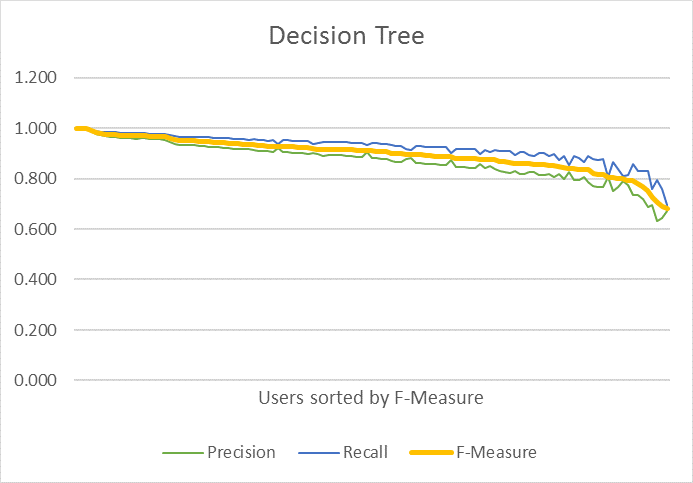
\includegraphics[width=\textwidth]{files/all_users_combined/decision_tree_stas_line}
		\end{minipage}
		\hfill
		\begin{minipage}[t]{0.69\textwidth}
			\centering
			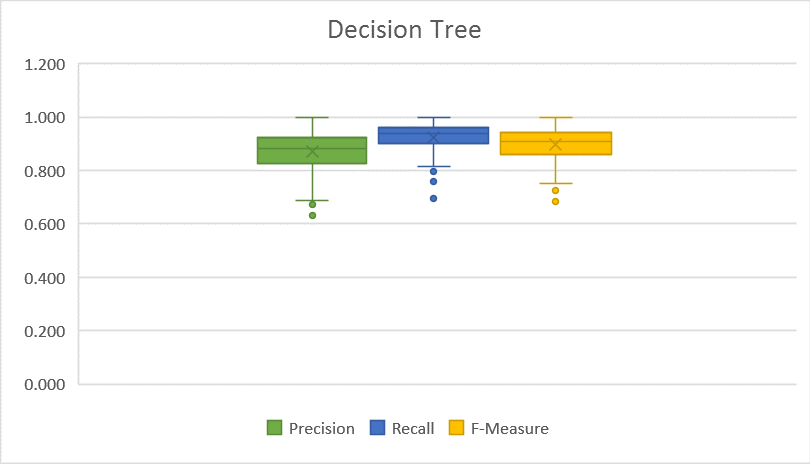
\includegraphics[width=\textwidth]{files/all_users_combined/decision_tree_stas_boxplot}
		\end{minipage}
		\hfill
	}
	\caption{Stations Features for Decision Tree}
\end{figure}

% Decision Tree - Current Station & Timestamp
\begin{figure}[H]
	\makebox[\textwidth]{
		\begin{minipage}[t]{0.7\textwidth}
			\centering
			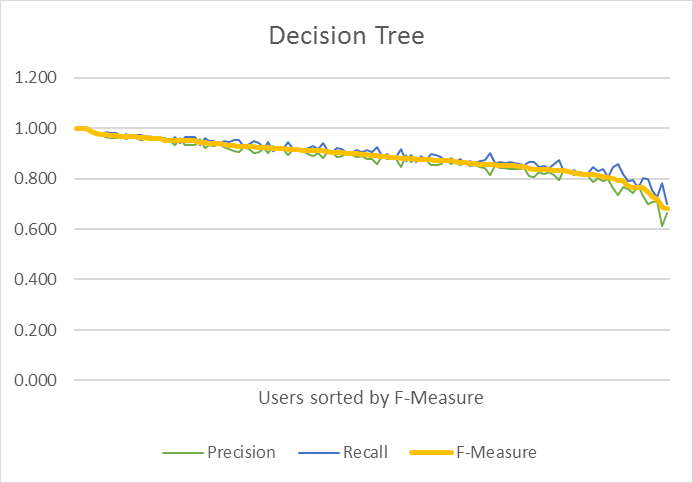
\includegraphics[width=\textwidth]{files/all_users_combined/decision_tree_csta_ts_line}
		\end{minipage}
		\hfill
		\begin{minipage}[t]{0.69\textwidth}
			\centering
			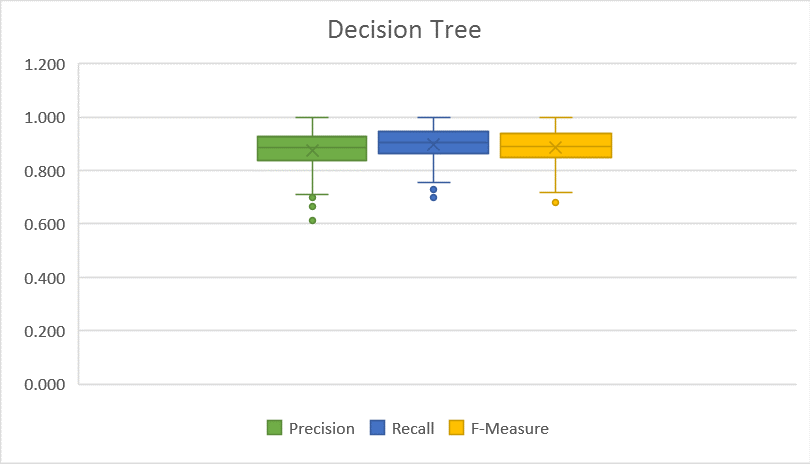
\includegraphics[width=\textwidth]{files/all_users_combined/decision_tree_csta_ts_boxplot}
		\end{minipage}
		\hfill
	}
	\caption{Current Station and Time-Based Features for Decision Tree}
\end{figure}

% Decision Tree - All Features
\begin{figure}[H]
	\makebox[\textwidth]{
		\begin{minipage}[t]{0.7\textwidth}
			\centering
			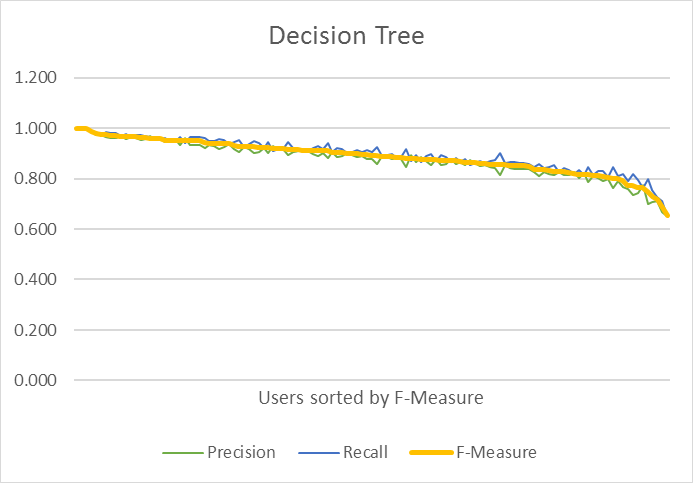
\includegraphics[width=\textwidth]{files/all_users_combined/decision_tree_all_line}
		\end{minipage}
		\hfill
		\begin{minipage}[t]{0.69\textwidth}
			\centering
			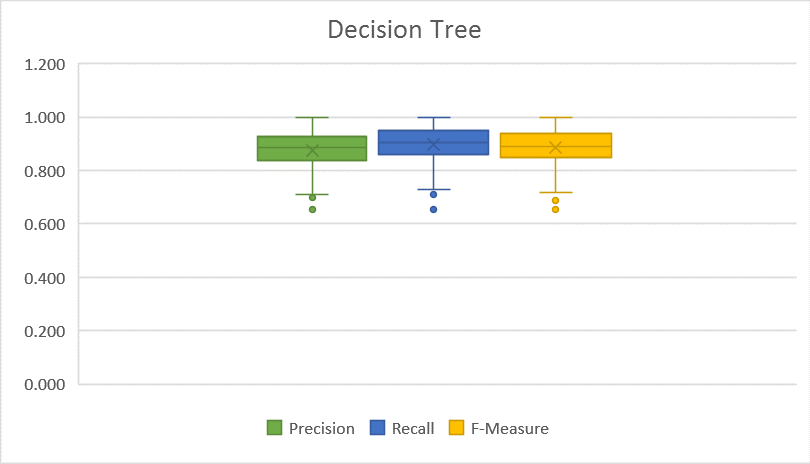
\includegraphics[width=\textwidth]{files/all_users_combined/decision_tree_all_boxplot}
		\end{minipage}
		\hfill
	}
	\caption{All Features for Decision Tree}
\end{figure}


\paragraphtitle{Naive Bayes}
% Naive Bayes - Stations
\begin{figure}[H]
	\makebox[\textwidth]{
		\begin{minipage}[t]{0.7\textwidth}
			\centering
			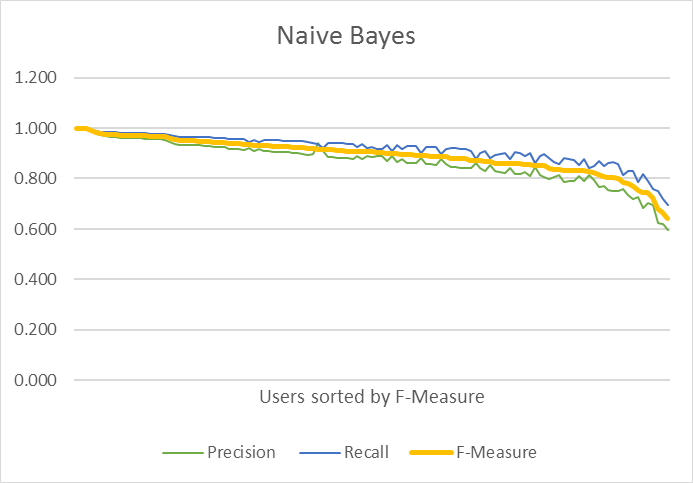
\includegraphics[width=\textwidth]{files/all_users_combined/naive_bayes_stas_line}
		\end{minipage}
		\hfill
		\begin{minipage}[t]{0.69\textwidth}
			\centering
			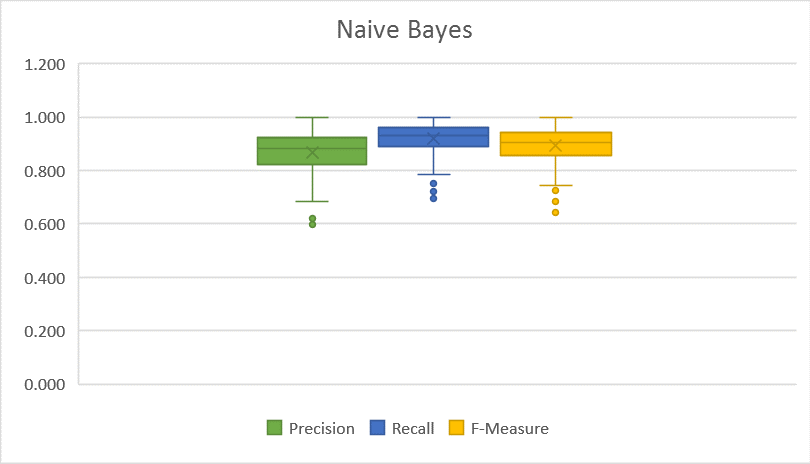
\includegraphics[width=\textwidth]{files/all_users_combined/naive_bayes_stas_boxplot}
		\end{minipage}
		\hfill
	}
	\caption{Stations Features for Naive Bayes}
\end{figure}

% Naive Bayes  - Current Station & Timestamp
\begin{figure}[H]
	\makebox[\textwidth]{
		\begin{minipage}[t]{0.7\textwidth}
			\centering
			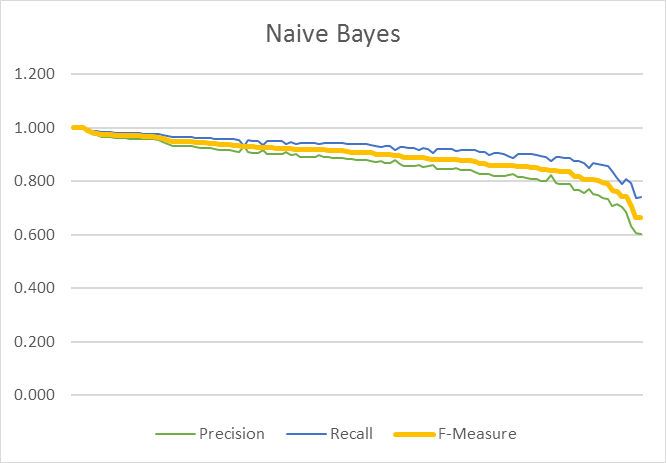
\includegraphics[width=\textwidth]{files/all_users_combined/naive_bayes_csta_ts_line}
		\end{minipage}
		\hfill
		\begin{minipage}[t]{0.69\textwidth}
			\centering
			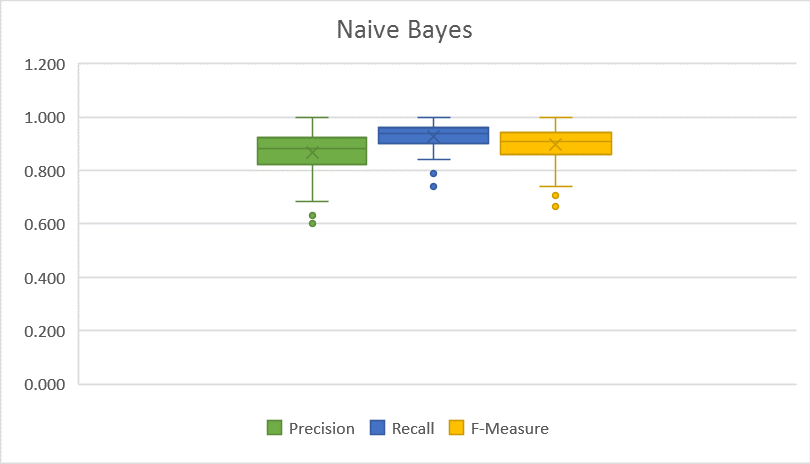
\includegraphics[width=\textwidth]{files/all_users_combined/naive_bayes_csta_ts_boxplot}
		\end{minipage}
		\hfill
	}
	\caption{Current Station and Time-Based Features for Naive Bayes}
\end{figure}

% Naive Bayes  - All Features
\begin{figure}[H]
	\makebox[\textwidth]{
		\begin{minipage}[t]{0.7\textwidth}
			\centering
			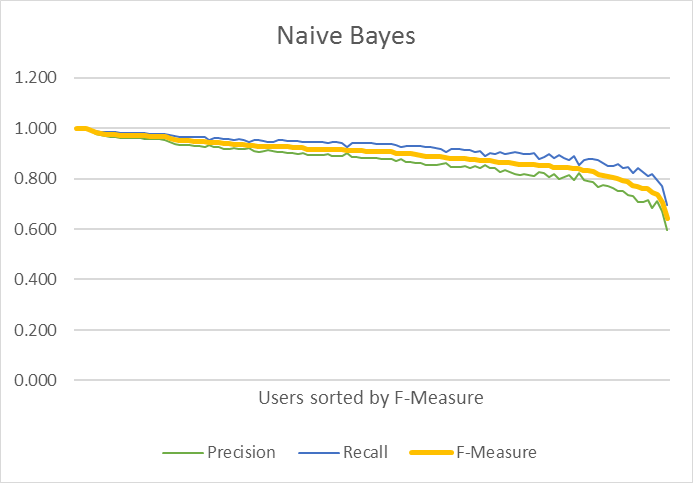
\includegraphics[width=\textwidth]{files/all_users_combined/naive_bayes_all_line}
		\end{minipage}
		\hfill
		\begin{minipage}[t]{0.69\textwidth}
			\centering
			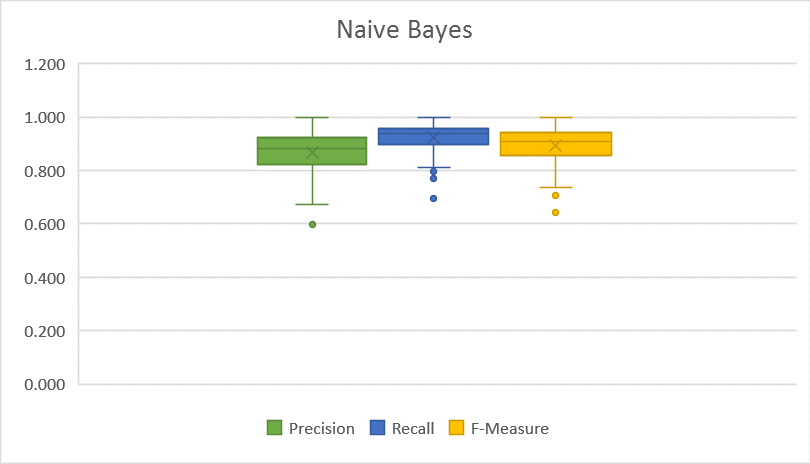
\includegraphics[width=\textwidth]{files/all_users_combined/naive_bayes_all_boxplot}
		\end{minipage}
		\hfill
	}
	\caption{All Features for Naive Bayes}
\end{figure}


\paragraphtitle{Multilayer Perceptron}
% Multilayer Perceptron - Stations
\begin{figure}[H]
	\makebox[\textwidth]{
		\begin{minipage}[t]{0.7\textwidth}
			\centering
			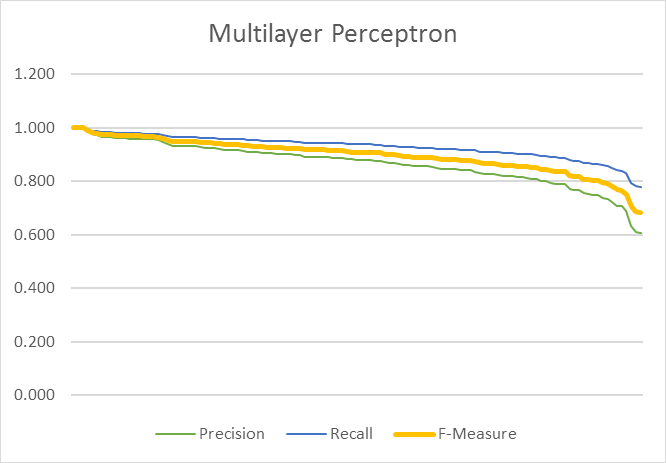
\includegraphics[width=\textwidth]{files/all_users_combined/mp_stas_line}
		\end{minipage}
		\hfill
		\begin{minipage}[t]{0.69\textwidth}
			\centering
			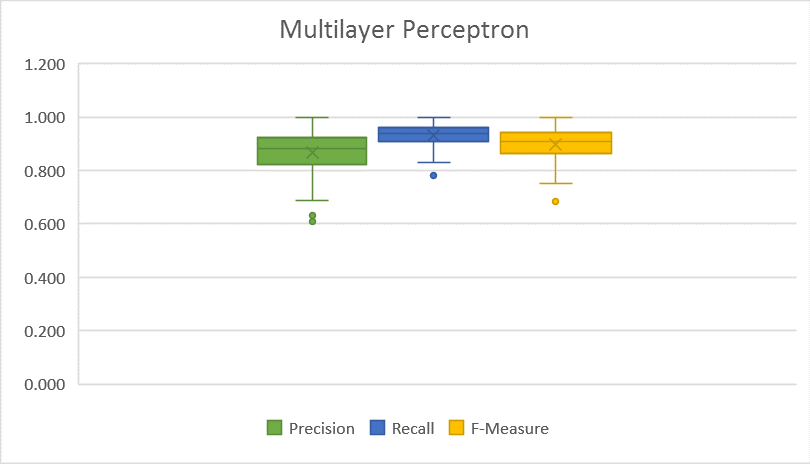
\includegraphics[width=\textwidth]{files/all_users_combined/mp_stas_boxplot}
		\end{minipage}
		\hfill
	}
	\caption{Stations Features for Multilayer Perceptron}
\end{figure}

% Multilayer Perceptron - Current Station & Timestamp
\begin{figure}[H]
	\makebox[\textwidth]{
		\begin{minipage}[t]{0.7\textwidth}
			\centering
			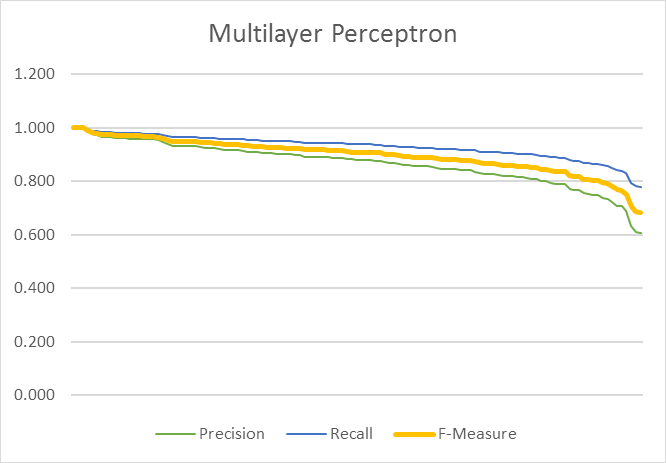
\includegraphics[width=\textwidth]{files/all_users_combined/mp_csta_ts_line}
		\end{minipage}
		\hfill
		\begin{minipage}[t]{0.69\textwidth}
			\centering
			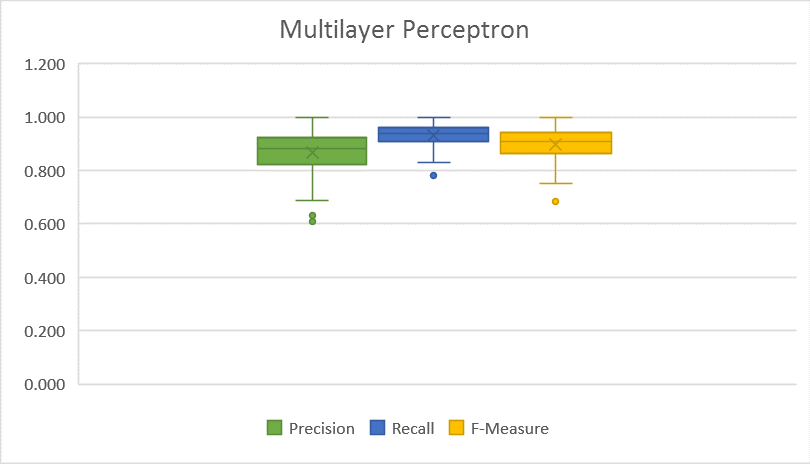
\includegraphics[width=\textwidth]{files/all_users_combined/mp_csta_ts_boxplot}
		\end{minipage}
		\hfill
	}
	\caption{Current Station and Time-Based Features for Multilayer Perceptron}
\end{figure}

% Multilayer Perceptron - All Features
\begin{figure}[H]
	\makebox[\textwidth]{
		\begin{minipage}[t]{0.7\textwidth}
			\centering
			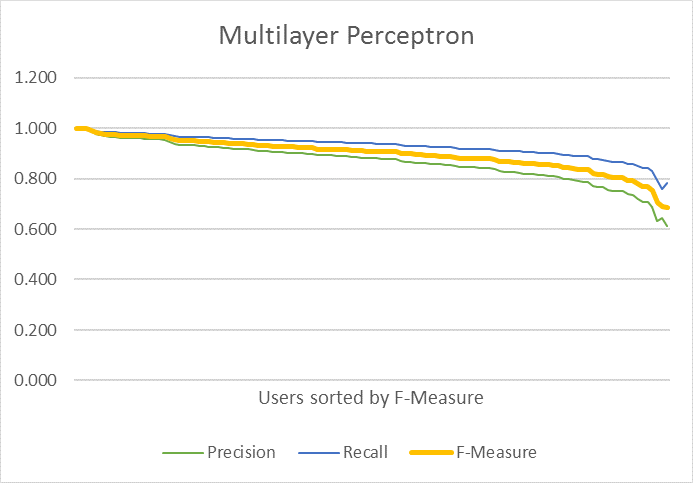
\includegraphics[width=\textwidth]{files/all_users_combined/mp_all_line}
		\end{minipage}
		\hfill
		\begin{minipage}[t]{0.69\textwidth}
			\centering
			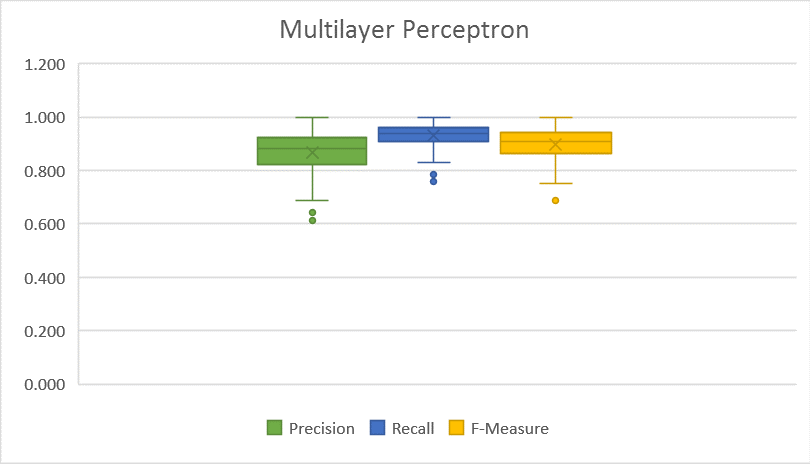
\includegraphics[width=\textwidth]{files/all_users_combined/mp_all_boxplot}
		\end{minipage}
		\hfill
	}
	\caption{All Features for Multilayer Perceptron}
\end{figure}


\newpage
\subsubsection{Comparison of frequent versus non-frequent Users}
In this experiment we have let the algorithm run through our data set as before, however before creating the graph for our evaluation we have split the result set into high- and low-frequency users. The split is done by 50\% of our data set. We simply count the number of data entries a user has to see whether that user belongs into the high- or low-frequency belt. In the graphs below the left-hand side of the graph represent the high-frequency users and the right-hand side the low-frequency users. Each half is then ordered by their respective F-Values just as before.

\paragraphtitle{Decision Trees}
% Decision Tree - Stations
\begin{figure}[H]
	\centering
	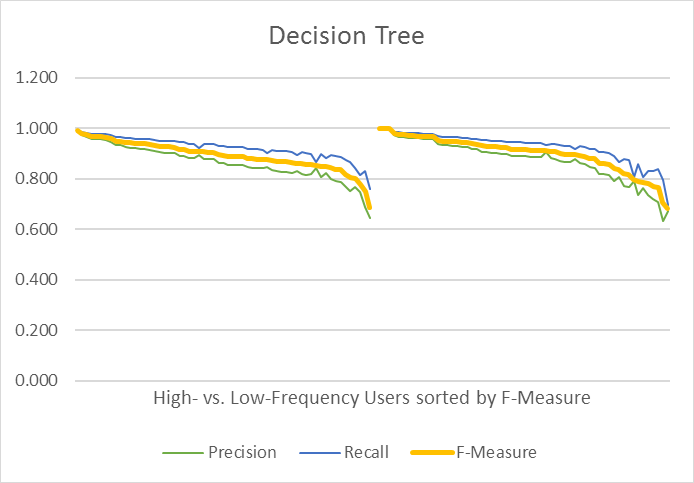
\includegraphics[width=0.7\textwidth]{files/high_vs_low_frequency/decision_tree_stas}
	\caption{Stations Features for Decision Tree}
\end{figure}

% Decision Tree - Current Station & Timestamp
\begin{figure}[H]
	\centering
	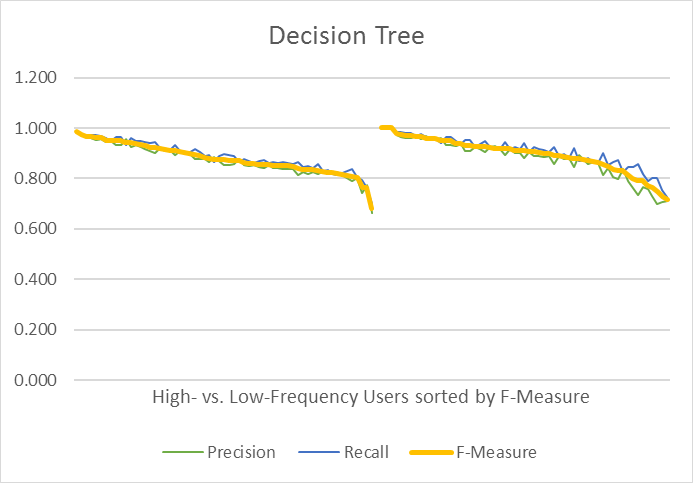
\includegraphics[width=0.7\textwidth]{files/high_vs_low_frequency/decision_tree_csta_ts}
	\caption{Current Station and Time-Based Features for Decision Tree}
\end{figure}

% Decision Tree - All Features
\begin{figure}[H]
	\centering
	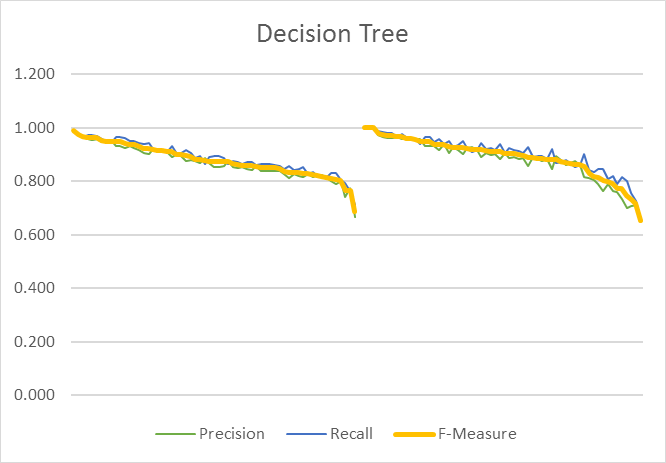
\includegraphics[width=0.7\textwidth]{files/high_vs_low_frequency/decision_tree_all}
	\caption{All Features for Decision Tree}
\end{figure}


\paragraphtitle{Naive Bayes}
% Naive Bayes - Stations
\begin{figure}[H]
	\centering
	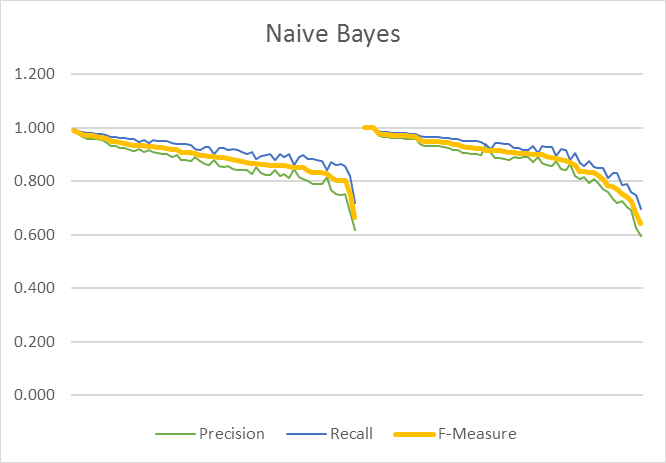
\includegraphics[width=0.7\textwidth]{files/high_vs_low_frequency/naive_bayes_stas}
	\caption{Stations Features for Naive Bayes}
\end{figure}

% Naive Bayes - Current Station & Timestamp
\begin{figure}[H]
	\centering
	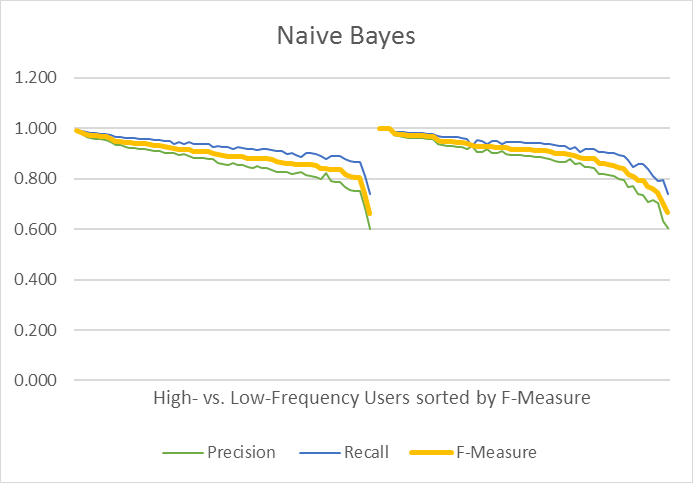
\includegraphics[width=0.7\textwidth]{files/high_vs_low_frequency/naive_bayes_csta_ts}
	\caption{Current Station and Time-Based Features for Naive Bayes}
\end{figure}

% Naive Bayes - All Features
\begin{figure}[H]
	\centering
	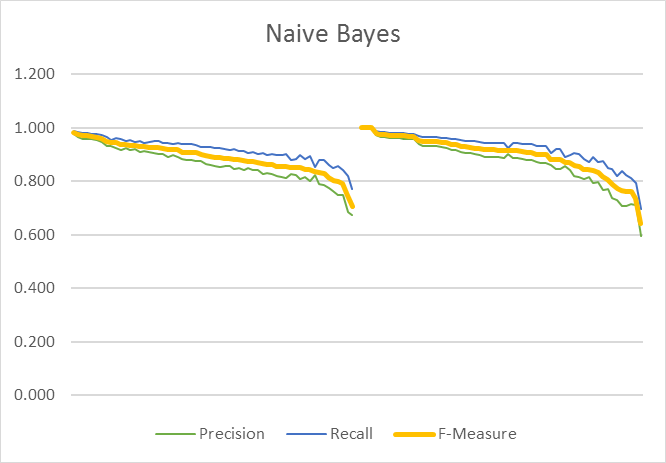
\includegraphics[width=0.7\textwidth]{files/high_vs_low_frequency/naive_bayes_all}
	\caption{All Features for Naive Bayes}
\end{figure}


\paragraphtitle{Multilayer Perceptron}
% Multilayer Perceptron - Stations
\begin{figure}[H]
	\centering
	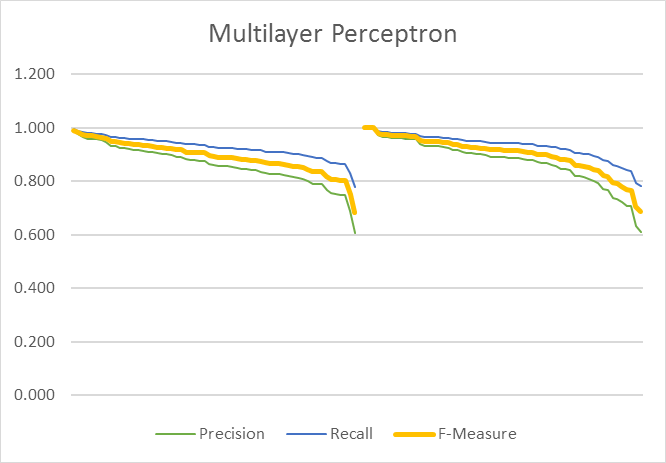
\includegraphics[width=0.7\textwidth]{files/high_vs_low_frequency/mp_stas}
	\caption{Stations Features for Multilayer Perceptron}
\end{figure}

% Multilayer Perceptron - Current Station & Timestamp
\begin{figure}[H]
	\centering
	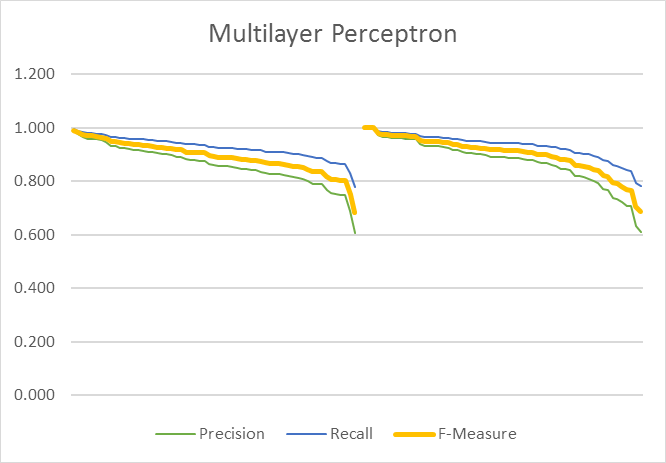
\includegraphics[width=0.7\textwidth]{files/high_vs_low_frequency/mp_csta_ts}
	\caption{Current Station and Time-Based Features for Multilayer Perceptron}
\end{figure}

% Multilayer Perceptron - All Features
\begin{figure}[H]
	\centering
	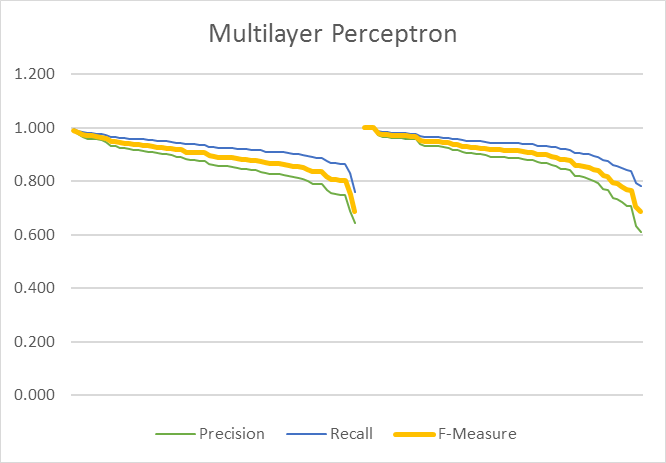
\includegraphics[width=0.7\textwidth]{files/high_vs_low_frequency/mp_all}
	\caption{All Features for Multilayer Perceptron}
\end{figure}


\newpage
\subsubsection{Comparison of all Users with higher number of Stations}
For our last experiment we have played a bit with the parameters of the number of stations we include in our prediction and the minimum amount of occurrences the stations have to have. The way its used is described in more detail in subsection \ref{subsubsec:data_preparation}. We ran the simulation multiple times with higher and lower thresholds to see what changes. We have taken two thresholds that represent the tests in a good way. In this experiment the maximum amount of stations is set to 15 whereas the necessary amount of occurrences is reduced to five. This has led to a steep increase in users that are actually processed (almost double). Due to the higher user count and the increased complexity, we have not included the Multilayer Perceptron Algorithm in this experiment. It was multiple orders of magnitudes slower and didn't yield significantly different results. 

\paragraphtitle{Decision Trees}
% Decision Tree - Stations
\begin{figure}[H]
	\makebox[\textwidth]{
		\begin{minipage}[t]{0.7\textwidth}
			\centering
			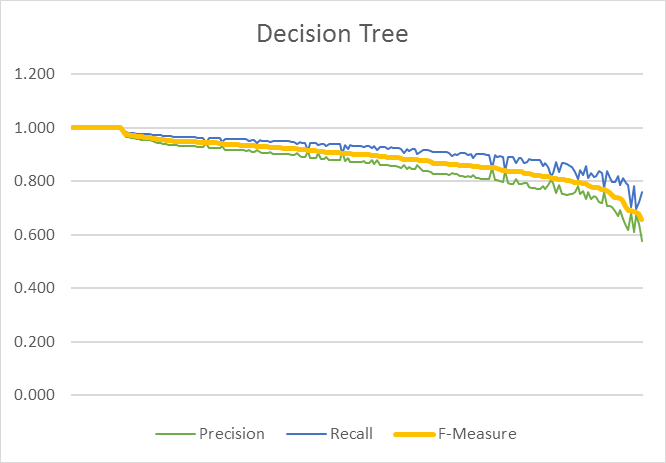
\includegraphics[width=\textwidth]{files/all_users_combined_more_station/decision_tree_stas_line}
		\end{minipage}
		\hfill
		\begin{minipage}[t]{0.69\textwidth}
			\centering
			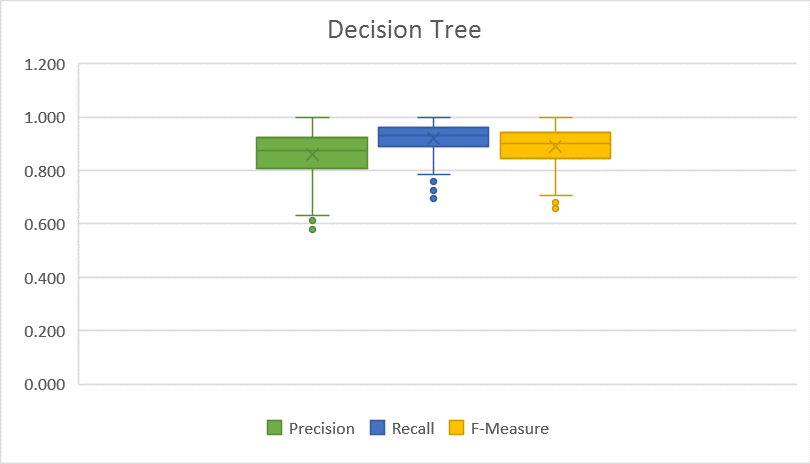
\includegraphics[width=\textwidth]{files/all_users_combined_more_station/decision_tree_stas_boxplot}
		\end{minipage}
		\hfill
	}
	\caption{Stations Features for Decision Tree}
\end{figure}

% Decision Tree - Current Station & Timestamp
\begin{figure}[H]
	\makebox[\textwidth]{
		\begin{minipage}[t]{0.7\textwidth}
			\centering
			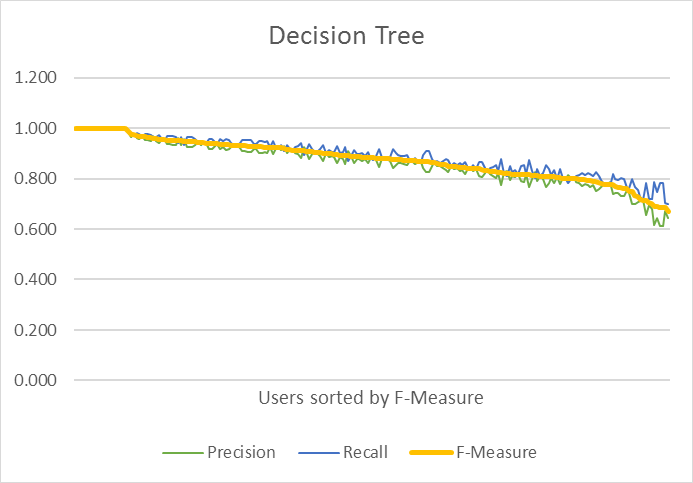
\includegraphics[width=\textwidth]{files/all_users_combined_more_station/decision_tree_csta_ts_line}
		\end{minipage}
		\hfill
		\begin{minipage}[t]{0.69\textwidth}
			\centering
			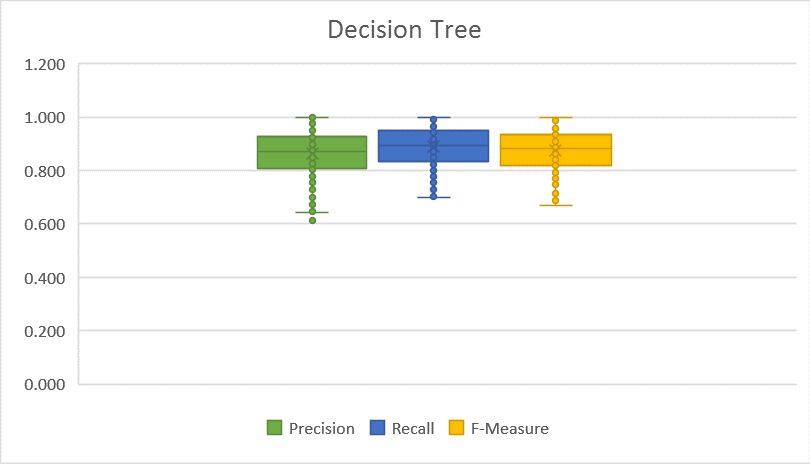
\includegraphics[width=\textwidth]{files/all_users_combined_more_station/decision_tree_csta_ts_boxplot}
		\end{minipage}
		\hfill
	}
	\caption{Current Station and Time-Based Features for Decision Tree}
\end{figure}

% Decision Tree - All Features
\begin{figure}[H]
	\makebox[\textwidth]{
		\begin{minipage}[t]{0.7\textwidth}
			\centering
			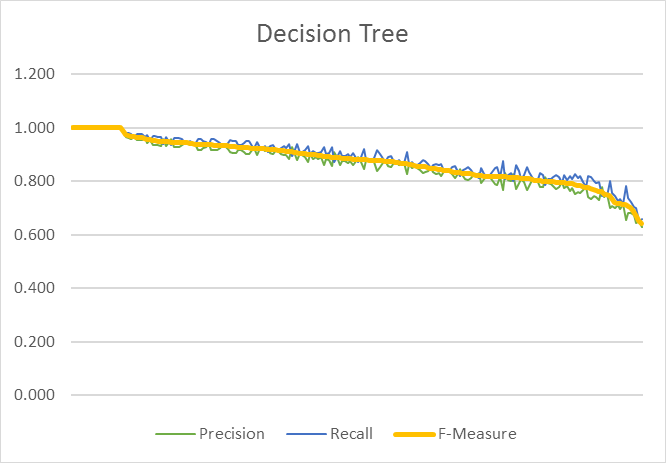
\includegraphics[width=\textwidth]{files/all_users_combined_more_station/decision_tree_all_line}
		\end{minipage}
		\hfill
		\begin{minipage}[t]{0.69\textwidth}
			\centering
			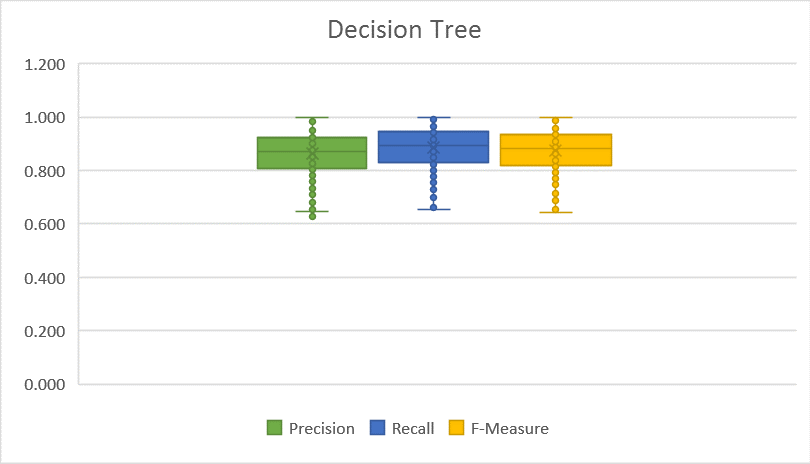
\includegraphics[width=\textwidth]{files/all_users_combined_more_station/decision_tree_all_boxplot}
		\end{minipage}
		\hfill
	}
	\caption{All Features for Decision Tree}
\end{figure}


\paragraphtitle{Naive Bayes}
% Naive Bayes - Stations
\begin{figure}[H]
	\makebox[\textwidth]{
		\begin{minipage}[t]{0.7\textwidth}
			\centering
			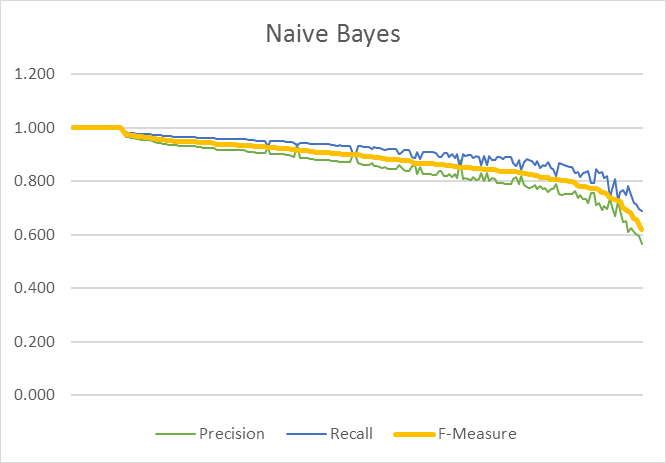
\includegraphics[width=\textwidth]{files/all_users_combined_more_station/naive_bayes_stas_line}
		\end{minipage}
		\hfill
		\begin{minipage}[t]{0.69\textwidth}
			\centering
			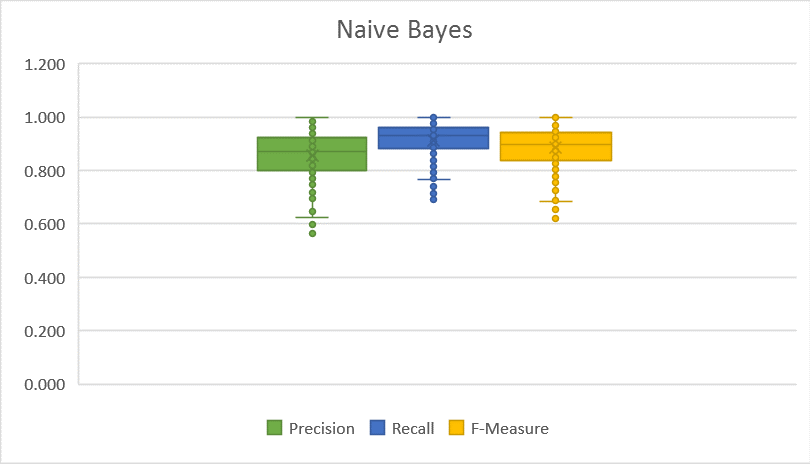
\includegraphics[width=\textwidth]{files/all_users_combined_more_station/naive_bayes_stas_boxplot}
		\end{minipage}
		\hfill
	}
	\caption{Stations Features for Naive Bayes}
\end{figure}

% Naive Bayes  - Current Station & Timestamp
\begin{figure}[H]
	\makebox[\textwidth]{
		\begin{minipage}[t]{0.7\textwidth}
			\centering
			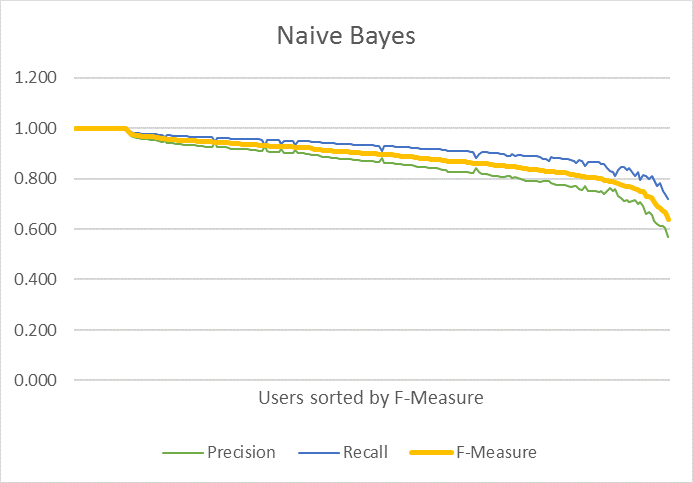
\includegraphics[width=\textwidth]{files/all_users_combined_more_station/naive_bayes_csta_ts_line}
		\end{minipage}
		\hfill
		\begin{minipage}[t]{0.69\textwidth}
			\centering
			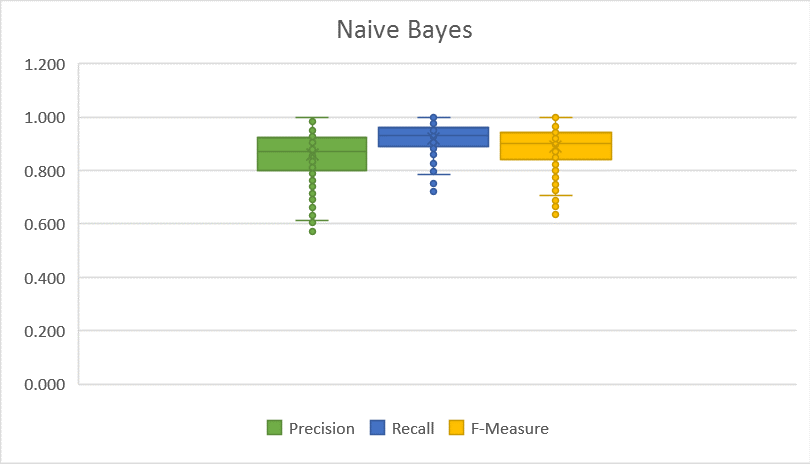
\includegraphics[width=\textwidth]{files/all_users_combined_more_station/naive_bayes_csta_ts_boxplot}
		\end{minipage}
		\hfill
	}
	\caption{Current Station and Time-Based Features for Naive Bayes}
\end{figure}

% Naive Bayes  - All Features
\begin{figure}[H]
	\makebox[\textwidth]{
		\begin{minipage}[t]{0.7\textwidth}
			\centering
			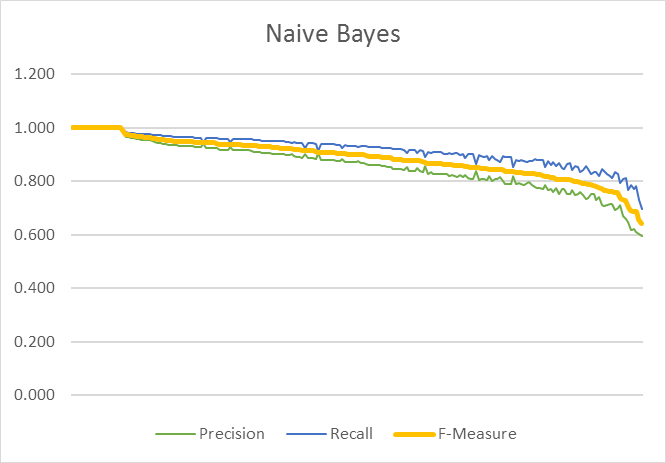
\includegraphics[width=\textwidth]{files/all_users_combined_more_station/naive_bayes_all_line}
		\end{minipage}
		\hfill
		\begin{minipage}[t]{0.69\textwidth}
			\centering
			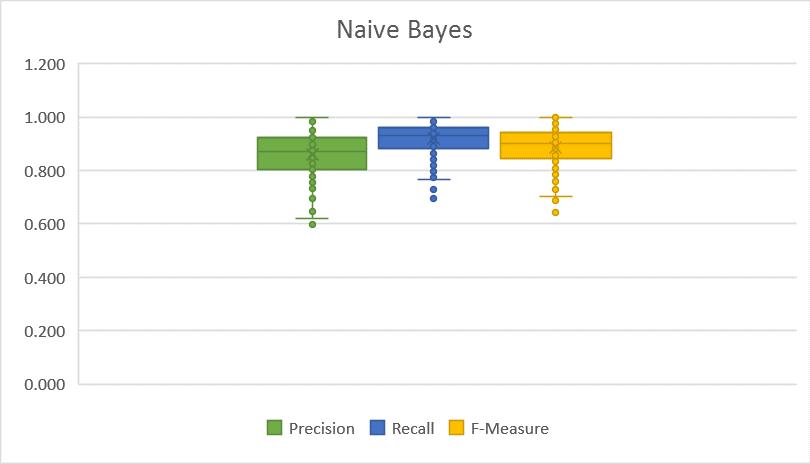
\includegraphics[width=\textwidth]{files/all_users_combined_more_station/naive_bayes_all_boxplot}
		\end{minipage}
		\hfill
	}
	\caption{All Features for Naive Bayes}
\end{figure}


\subsection{Comparison of Results}

\subsubsection{Comparison of different algorithms}
In general it can be said that the selection of the machine learning algorithm hasn't heavily influenced the final results. The F-Measure is quite similar in all of the algorithms, given the same feature set. What is quite different in the algorithms is the consistency of how precision and recall correlate. In our Multilayer Perceptron experiments the precision and recall lines are a lot smoother, meaning that they deteriorate in combination and are quite stable across all users. Recall is usually higher than precision, but the difference between them is stable. This was also apparent between the different feature set. For Naive Bayes and to an even larger extent the decision tree algorithm the curves for precision and recall have lots of small mountains and valleys, especially when looking at the results with lower precision. This leads to the conclusion that the results are more dependent on the specific data for the Naive Bayes and Decision Tree algorithms and we might have some over- or underfitting for these algorithms. The overall precision hasn't suffered too much, but the Multilayer Perceptron algorithm is certainly the most stable of all.

For all algorithms we have experienced a relative straight line up unto approximately 85-90\% of the users where we see a quite sharp decline. For those users it might be interesting to check with a different algorithm and see whether the results are similarly low. If the precision doesn't get better we would most likely need to filter them out until more and especially more precise data has been gathered. Because a precision and recall of around 0.7 generally doesn't give us a big benefit. However for about 50\% of our users in all algorithms we have a F-Measure of 0.9, which could probably be used in a production system. Combined with some feedback from the actual user that then explicitly validate our ground truth we can most likely eliminate or at least reduce our false predictions for our already high precision use cases.

\subsubsection{Comparison of different feature sets}
The overall difference between the different feature sets is also quite small. Especially when looking at the F-Measure curve, they show quite similar results, including the difference in algorithms. An interesting observation is that with the addition of time-based features the precision and recall for the decision tree algorithm are a lot closer. The overall F-Measure is comparable, but the difference in precision and recall is smaller. The same change also includes quite a bit of stability for the Naive Bayes algorithm, smoothing out the precision and recall curve. The Multilayer Perceptron didn't show much difference, only some small inconsistencies at the tail of the curve. However since the Multilayer Perceptron is already quite stable the addition of time-based features hasn't helped much.

The distribution of values (from our boxplot charts) across the feature sets are also quite similar. The precision and F-Measure are mostly similarly distributed for each algorithm, the recall is varying a bit. Mostly it is the extrem values that vary, albeit only the lower ones, as the upper extremes are always 1.0. For the recall of the Decision Tree and Naive Bayes however we also see slight changes in the overall distribution. These effects cannot really be attested for the Multilayer Perceptron.

\subsubsection{Comparison of different experiments}
We can mostly compare the first and third experiment and separately see how the results of the second experiment differ and how they could benefit our overall prediction model.
The first experiment is quite conservative in the amount of data that are actually used in our machine learning algorithm. This is based on the assumptions that the algorithms can't cover all the special cases of our data and that the overall precision heavily benefits from our preprocessing and filtering. The third experiment also build upon some parts of this preprocessing and filtering, it is however far less restrictive, thus allowing a lot more and also a lot more low-frequency user to be included in our machine learning process. The results between those two experiments have shown what was to be expected. We have a much higher spread in our third experiment between the highest and the lowest F-Measures. The overall precision and recall are also a bit lower, however not by a huge margin. One of the interesting conclusion is that our third experiment had a lot more perfect predictions (precision = recall = F-Measure = 1.0). This can most likely be attributed to the fact that some low profile users are really easy to predict, if they have very few stations that they have used. Some of these users have already been filtered out in our first experiment. Whether these predictions would also hold up in reality or whether they can just be attributed to our data set is another question that can't be answered by our models. 

The issue with using the third experiment is that since the prediction for many more users fall below a usable threshold a lot more data needs to be discarded after our somewhat expensive machine learning calculations. Already filtering theses users out before we send the data through the machine learning system saves time and resources, all the while not generating a hugely negative impact on many of the users. Therefore it might make more sense to go with the first experiment or to use a combination of both, allowing the parameters to be set a bit more flexible for different users.

The second experiment is split in itself and compares high-frequency with low-frequency users. In the test data that we had the split was around 85 actually usable data entries (without all the removed entries from our preprocessing steps). Interestingly enough the curves looked very similar for both high- and low-frequency users. Both had a very sharp decline in the tail of the curve and otherwise quite consistent results. The decline is a bit more pronounced in the high-frequency users. This might help when trying to cut out the lowest X\% of the user set. But the overall prediction, recall and F-Measure values are very similar. It seems that when the users reach a certain amount of data entries it's not necessarily the pure amount of data that actually helps with the prediction, but a combination of other factors, such as the complexity of the data, the amount of different stations and the temporal distribution of the values.